% Seminarul 7: Cointegrare și VECM
% Serii de timp -- Programele de licență Informatică economică și Cibernetică economică, Academia de Studii Economice din București
% GENERAT de latex/build_seminar7.py -- modificați generatorul, nu acest fișier.
% Implicit versiunea pentru studenți; versiunea profesorului este wrapper-ul *_solutions.tex.
\makeatletter\@ifundefined{ifsolutions}{\expandafter\newif\csname ifsolutions\endcsname}{}\makeatother

\newcommand{\coursename}{Serii de timp}
\def\tsalang{ro}
% Preambul comun TSA -- Serii de timp / Time Series Analysis (Beamer, 16:9)
% Același design ca MFM și SFM (preluat din SFM, 5 octombrie 2026). Înainte de % Preambul comun TSA -- Serii de timp / Time Series Analysis (Beamer, 16:9)
% Același design ca MFM și SFM (preluat din SFM, 5 octombrie 2026). Înainte de % Preambul comun TSA -- Serii de timp / Time Series Analysis (Beamer, 16:9)
% Același design ca MFM și SFM (preluat din SFM, 5 octombrie 2026). Înainte de \input{../../latex/preamble} se definește
%   \newcommand{\coursename}{Time Series Analysis}      (EN)
%   \newcommand{\coursename}{Serii de timp}       (RO)  și  \def\tsalang{ro}
% Fișierele .tex se află în EN/Courses, EN/Seminars, RO/Cursuri, RO/Seminarii (două niveluri sub rădăcină).
% Deck-urile sînt generate de latex/build_chapterN.py / build_seminarN.py (vezi latex/tsa_build.py).

\documentclass[9pt, aspectratio=169, t]{beamer}
\providecommand{\coursename}{Time Series Analysis}

% Ensure content fits on slides
\setbeamersize{text margin left=8mm, text margin right=8mm}
% Smaller institute font (title page)
\setbeamerfont{institute}{size=\footnotesize}

%=============================================================================
% THEME AND STYLE CONFIGURATION
%=============================================================================
\usetheme{default}
% Using default theme for clean header/footer control

% Color Palette (matching Redispatch PDF)
\definecolor{MainBlue}{RGB}{26, 58, 110}
\definecolor{AccentBlue}{RGB}{26, 58, 110}
\definecolor{IDAred}{RGB}{205, 0, 0}
\definecolor{DarkGray}{RGB}{51, 51, 51}
\definecolor{MediumGray}{RGB}{128, 128, 128}
\definecolor{LightGray}{RGB}{248, 248, 248}
\definecolor{VeryLightGray}{RGB}{235, 235, 235}
\definecolor{KeynoteGray}{RGB}{218, 218, 218}
\definecolor{SectionGray}{RGB}{120, 120, 120}
\definecolor{FooterGray}{RGB}{100, 100, 100}
\definecolor{Crimson}{RGB}{220, 53, 69}
\definecolor{Forest}{RGB}{46, 125, 50}
\definecolor{Amber}{RGB}{181, 133, 63}
\definecolor{Orange}{RGB}{230, 126, 34}
\definecolor{Purple}{RGB}{142, 68, 173}

% Gradient background (exact Keynote 315° gradient: white to RGB 218,218,218)
\setbeamertemplate{background}{%
    \begin{tikzpicture}[remember picture, overlay]
        \shade[shading=axis, shading angle=315,
        top color=white, bottom color=KeynoteGray]
        (current page.south west) rectangle (current page.north east);
    \end{tikzpicture}%
}
% Fallback solid color for compatibility
\setbeamercolor{background canvas}{bg=}

\setbeamercolor{palette primary}{bg=MainBlue, fg=white}
\setbeamercolor{palette secondary}{bg=MainBlue!85, fg=white}
\setbeamercolor{palette tertiary}{bg=MainBlue!70, fg=white}
\setbeamercolor{structure}{fg=MainBlue}
\setbeamercolor{title}{fg=IDAred}
\setbeamercolor{frametitle}{fg=IDAred, bg=}
\setbeamercolor{block title}{bg=MainBlue, fg=white}
\setbeamercolor{block body}{bg=VeryLightGray, fg=DarkGray}
\setbeamercolor{block title alerted}{bg=Crimson, fg=white}
\setbeamercolor{block body alerted}{bg=Crimson!8, fg=DarkGray}
\setbeamercolor{block title example}{bg=Forest, fg=white}
\setbeamercolor{block body example}{bg=Forest!8, fg=DarkGray}
\setbeamercolor{item}{fg=MainBlue}

% Footer colors (override Madrid theme blue)
\setbeamercolor{author in head/foot}{fg=FooterGray, bg=}
\setbeamercolor{title in head/foot}{fg=FooterGray, bg=}
\setbeamercolor{date in head/foot}{fg=FooterGray, bg=}
\setbeamercolor{section in head/foot}{fg=FooterGray, bg=}
\setbeamercolor{subsection in head/foot}{fg=FooterGray, bg=}

% Bullet styles (apply everywhere including blocks)
\setbeamertemplate{itemize item}{\color{MainBlue}$\boxdot$}
\setbeamertemplate{itemize subitem}{\color{MainBlue}$\blacktriangleright$}
\setbeamertemplate{itemize subsubitem}{\color{MainBlue}\tiny$\bullet$}
\setbeamertemplate{itemize/enumerate body begin}{\normalsize}
\setbeamertemplate{itemize/enumerate subbody begin}{\normalsize}

% Item spacing - compact style
\setlength{\leftmargini}{10pt}       % Level 1: minimal indent
\setlength{\leftmarginii}{10pt}      % Level 2: minimal additional indent
% Compact list spacing (zero extra space before/after lists in blocks)
\makeatletter
\def\@listi{\leftmargin\leftmargini \topsep 0pt \parsep 0pt \itemsep 0pt}
\def\@listii{\leftmargin\leftmarginii \topsep 0pt \parsep 0pt \itemsep 0pt}
\makeatother

\setbeamertemplate{navigation symbols}{}

%=============================================================================
% CUSTOM HEADLINE
%=============================================================================
\setbeamertemplate{headline}{%
    \vskip10pt%
    \hbox to \paperwidth{%
        \hskip0.5cm%
        {\small\color{FooterGray}\renewcommand{\hyperlink}[2]{##2}\insertsectionhead}%
        \hfill%
        \textcolor{FooterGray}{\small\insertframenumber}%
        \hskip0.5cm%
    }%
    \vskip4pt%
    {\color{FooterGray}\hrule height 0.4pt}%
}

%=============================================================================
% CUSTOM FOOTER
%=============================================================================
\usepackage{fontawesome5}

\setbeamertemplate{footline}{%
    {\color{FooterGray}\hrule height 0.4pt}%
    \vskip4pt%
    \hbox to \paperwidth{%
        \hskip0.5cm%
        \textcolor{FooterGray}{\small\coursename}%
        \hfill%
        \raisebox{-0.1em}{%
            \begin{tikzpicture}[x=0.08em, y=0.08em, line width=0.4pt]
                \draw[FooterGray] (0,3) -- (1,4) -- (2,3.5) -- (3,5) -- (4,4) -- (5,6) -- (6,5.5) -- (7,4) -- (8,5) -- (9,7) -- (10,6) -- (11,5) -- (12,6.5) -- (13,8) -- (14,7) -- (15,6) -- (16,7.5) -- (17,9) -- (18,8) -- (19,7) -- (20,8.5) -- (21,10) -- (22,9) -- (23,8) -- (24,9.5);
            \end{tikzpicture}%
        }%
        \hskip0.5cm%
    }%
    \vskip6pt%
}

%=============================================================================
% PACKAGES
%=============================================================================
\usepackage[utf8]{inputenc}
\DeclareUnicodeCharacter{03B1}{\ensuremath{\alpha}}
\usepackage[T1]{fontenc}
\usepackage{amsmath, amssymb, amsthm}
\usepackage{mathtools}
\usepackage{bm}
\usepackage{tikz}
\usetikzlibrary{arrows.meta, positioning, shapes, calc, decorations.pathreplacing, shadings}
\usepackage{booktabs}
\usepackage{multirow}
\usepackage{array}
\usepackage{graphicx}
\usepackage{animate}
\usepackage{hyperref}
\usepackage{colortbl}
\usepackage{listings}
\lstset{language=Python, basicstyle=\ttfamily\scriptsize, keywordstyle=\color{MainBlue}\bfseries,
  commentstyle=\color{Forest}, stringstyle=\color{Crimson}, breaklines=true,
  frame=none, backgroundcolor=\color{VeryLightGray}, xleftmargin=2mm}
\hypersetup{colorlinks=true, linkcolor=MainBlue, urlcolor=MainBlue}
\graphicspath{{../../logos/}{../../charts/}{../../photos/}}
\usepackage{xcolor}
\hfuzz=2pt  % Suppress tiny overfull warnings (<2pt)
\vfuzz=2pt  % Suppress tiny vertical overfull warnings (<2pt)
% \mathrm in the sans-serif family of the slides (beamer resets \mathrm to the serif family at \begin{document};
% this hook runs after beamer's, so WN, Var, RMSE, ... in formulas match the surrounding text)
% Bold vectors and matrices in the same sans-serif family: \mathbf{A} in sans bold (beamer's own \mathbf came out in
% medium weight), and the bold upright Greek capitals of \boldsymbol / \bm (\bSigma, \bPhi, \boldsymbol{\Theta}) in
% cmss bold: bm.sty fixes its "boldoperators" font when it is loaded (serif cmbx), before beamer switches the
% operators to cmss, so it is reset here.
\AtBeginDocument{%
  \SetMathAlphabet{\mathrm}{normal}{\encodingdefault}{\sfdefault}{\mddefault}{n}%
  \SetMathAlphabet{\mathrm}{bold}{\encodingdefault}{\sfdefault}{bx}{n}%
  \SetMathAlphabet{\mathbf}{normal}{\encodingdefault}{\sfdefault}{bx}{n}%
  \SetMathAlphabet{\mathbf}{bold}{\encodingdefault}{\sfdefault}{bx}{n}%
  \SetSymbolFont{boldoperators}{normal}{OT1}{cmss}{bx}{n}%
  \SetSymbolFont{boldoperators}{bold}{OT1}{cmss}{bx}{n}}

%=============================================================================
% QUANTLET COMMANDS
%   \quantlet{<displayed name>}{<url>}       (generic, compatible with the older TSA decks)
%   \tsaquantlet{Ch_05}{TSA_ch5_garch}       -> https://github.com/danpele/Time-Series-Analysis/tree/main/Quantlets/Ch_05/TSA_ch5_garch
%   \qlurl{<folder>} is defined per chapter by the generator (Quantlets/Ch_NN/<folder>)
%=============================================================================
\newcommand{\tsarepo}{https://github.com/danpele/Time-Series-Analysis}
\newcommand{\tsaqlbase}{https://github.com/danpele/Time-Series-Analysis/tree/main/Quantlets}
\newcommand{\quantlet}[2]{%
    \hfill\href{#2}{%
        \raisebox{-0.15em}{
\includegraphics[height=0.7em]{ql_logo.png}}%
        \textcolor{MainBlue}{\tiny\ #1}%
    }%
}
\newcommand{\tsaquantlet}[2]{\quantlet{\detokenize{#2}}{\tsaqlbase/#1/#2}}

%=============================================================================
% NOTEBOOKS (Google Colab)
%   \colaburl{notebooks/EN/chapter5_seminar_notebook.ipynb} -> the Colab link of a file in the TSA repo
%   \nb: the chapter notebook (each seminar deck redefines it with \renewcommand)
%=============================================================================
\newcommand{\colaburl}[1]{https://colab.research.google.com/github/danpele/Time-Series-Analysis/blob/main/#1}
\newcommand{\nb}{https://colab.research.google.com/github/danpele/Time-Series-Analysis/tree/main/notebooks/EN}
\newcommand{\nbname}{notebooks/EN}

%=============================================================================
% SLIDE HELPERS (used by the generators; the same as in MFM)
%=============================================================================
% local font size for list bodies (the preamble forces \normalsize)
\newcommand{\itemsize}[1]{\setbeamertemplate{itemize/enumerate body begin}{#1}\setbeamertemplate{itemize/enumerate subbody begin}{#1}}
\newcommand{\intitle}[1]{{\hypersetup{urlcolor=white}#1}}   % white links inside coloured title bars
\newcommand{\imgcap}[1]{{\scriptsize #1}\\[0.5mm]}          % caption under a photo
\newcommand{\imgcredit}[2]{{\tiny\color{FooterGray}\href{#1}{#2}}}   % image credit: source URL, author/licence
\newcommand{\aiprompt}[1]{{\ttfamily\color{MainBlue}#1}}     % a prompt to an AI assistant

%=============================================================================
% SEMINARS: student version by default; the instructor wrapper *_solutions.tex sets \solutionstrue
%=============================================================================
\makeatletter\@ifundefined{ifsolutions}{\expandafter\newif\csname ifsolutions\endcsname}{}\makeatother
\newcommand{\solonly}[1]{\ifsolutions #1\fi}
\newcommand{\propsub}{\ifsolutions\else\framesubtitle{\ifdefined\tsalang Rezolvarea se discută la seminar\else Solution discussed in class\fi}\fi}

%=============================================================================
% APPENDIX AND CHAPTER LINKS (latex/appendix_links.py writes the calls; it also re-declares these
% macros before \begin{document}, so the decks compile with or without this preamble block)
%=============================================================================
\providecommand{\tsaapplink}[3]{\hypertarget{#2}{}\hyperlink{#1}{\beamergotobutton{#3}}}
\providecommand{\tsaappback}[2]{\begin{tikzpicture}[remember picture,overlay]\node[anchor=south east] at ([xshift=-3mm,yshift=7mm]current page.south east){\hyperlink{#1}{\beamerreturnbutton{#2}}};\end{tikzpicture}}
\providecommand{\tsachlink}[2]{\href{#1}{#2}}
\providecommand{\tsachlinkt}[2]{\href{#1}{\usebeamercolor[fg]{frametitle}#2}}

%=============================================================================
% QUANTINAR COMMAND: link către un curs Quantinar (subiecte avansate)
%=============================================================================
\newcommand{\quantinar}[2]{%
    \href{#2}{%
        \raisebox{-0.15em}{
\includegraphics[height=0.8em]{qr_logo.png}}%
        \textcolor{MainBlue}{\scriptsize\ #1}%
    }%
}

%=============================================================================
% CUSTOM TITLE PAGE
%=============================================================================
\defbeamertemplate*{title page}{hybrid}[1][]
{
    \vspace{0.2cm}
    % Logos row - top header (with clickable links)
    \begin{center}
        \href{https://www.ase.ro}{
\includegraphics[height=1.0cm]{ase_logo.png}}\hspace{0.3cm}%
        \href{https://theida.net}{
\includegraphics[height=1.0cm]{ida_logo.png}}\hspace{0.3cm}%
        \href{https://blockchain-research-center.com}{
\includegraphics[height=1.0cm]{brc_logo.png}}\hspace{0.3cm}%
        \href{https://www.ai4efin.ase.ro}{
\includegraphics[height=1.0cm]{ai4efin_logo.png}}\hspace{0.3cm}%
        \href{https://ipe.ro/new}{
\includegraphics[height=1.0cm]{acad_logo.png}}\hspace{0.3cm}%
        \href{https://www.digital-finance-msca.com}{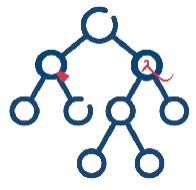
\includegraphics[height=1.0cm]{msca_logo.png}}%
    \end{center}

    \vspace{0.6cm}

    % Main title with Q logos on sides (with clickable links)
    \begin{center}
        \begin{minipage}{0.1\textwidth}
            \centering
            \href{https://quantlet.com}{
\includegraphics[height=1.1cm]{ql_logo.png}}
        \end{minipage}%
        \begin{minipage}{0.78\textwidth}
            \centering
            {\LARGE\bfseries\usebeamercolor[fg]{title}\inserttitle}

            \vspace{0.3cm}

            {\usebeamerfont{subtitle}\usebeamercolor[fg]{title}\insertsubtitle}
        \end{minipage}%
        \begin{minipage}{0.1\textwidth}
            \centering
            \href{https://quantinar.com}{
\includegraphics[height=1.1cm]{qr_logo.png}}
        \end{minipage}
    \end{center}

    \vspace{0.6cm}

    % Authors (left aligned)
    \hspace{0.5cm}{\usebeamerfont{author}\insertauthor}

    \vspace{0.3cm}

    % Institute/Affiliations (left aligned)
    \hspace{0.5cm}\begin{minipage}[t]{0.9\textwidth}
        \raggedright\small\insertinstitute
    \end{minipage}
}

%=============================================================================
% THEOREM ENVIRONMENTS
%=============================================================================
\theoremstyle{definition}
\setbeamertemplate{theorems}[numbered]
\ifdefined\tsalang
\newtheorem{defn}{Definiție}
\newtheorem{thm}{Teoremă}
\newtheorem{prop}{Propoziție}
\newtheorem{rmk}{Observație}
\else
\newtheorem{defn}{Definition}
\newtheorem{thm}{Theorem}
\newtheorem{prop}{Proposition}
\newtheorem{rmk}{Remark}
\fi

%=============================================================================
% CENTRED MINIPAGE (no extra vertical space)
%=============================================================================
\newenvironment{cminipage}[1]{%
    \par\noindent\hfill\begin{minipage}{#1}\ignorespaces
}{%
    \end{minipage}\hfill\null\par
}

%=============================================================================
% CUSTOM COMMANDS
%=============================================================================
\newcommand{\E}{\mathbb{E}}
\newcommand{\Var}{\text{Var}}
\newcommand{\Cov}{\text{Cov}}
\newcommand{\Corr}{\text{Corr}}
\newcommand{\R}{\mathbb{R}}
\newcommand{\N}{\mathbb{N}}
\newcommand{\Z}{\mathbb{Z}}
\newcommand{\B}{\mathbf{B}}
\newcommand{\imark}{\textcolor{MainBlue}{\textbullet}}
\newcommand{\RMSE}{\text{RMSE}}
\newcommand{\MAE}{\text{MAE}}
\newcommand{\MAPE}{\text{MAPE}}

% Boldface vector/matrix commands (VAR, VECM, state space; also used by the older TSA decks)
\newcommand{\bY}{\mathbf{Y}}
\newcommand{\bX}{\mathbf{X}}
\newcommand{\bA}{\mathbf{A}}
\newcommand{\bB}{\mathbf{B}}
\newcommand{\bepsilon}{\boldsymbol{\varepsilon}}
\newcommand{\bSigma}{\boldsymbol{\Sigma}}
\newcommand{\bPhi}{\boldsymbol{\Phi}}
\newcommand{\bGamma}{\boldsymbol{\Gamma}}
\newcommand{\bPi}{\boldsymbol{\Pi}}
\newcommand{\bc}{\mathbf{c}}
\newcommand{\balpha}{\boldsymbol{\alpha}}
\newcommand{\bbeta}{\boldsymbol{\beta}}
\newcommand{\bvarepsilon}{\boldsymbol{\varepsilon}}

% Legacy seminar marks (older TSA seminar decks)
\newcommand{\correct}{\textcolor{Forest}{\checkmark}}
\newcommand{\incorrect}{\textcolor{Crimson}{\texttimes}}
 se definește
%   \newcommand{\coursename}{Time Series Analysis}      (EN)
%   \newcommand{\coursename}{Serii de timp}       (RO)  și  \def\tsalang{ro}
% Fișierele .tex se află în EN/Courses, EN/Seminars, RO/Cursuri, RO/Seminarii (două niveluri sub rădăcină).
% Deck-urile sînt generate de latex/build_chapterN.py / build_seminarN.py (vezi latex/tsa_build.py).

\documentclass[9pt, aspectratio=169, t]{beamer}
\providecommand{\coursename}{Time Series Analysis}

% Ensure content fits on slides
\setbeamersize{text margin left=8mm, text margin right=8mm}
% Smaller institute font (title page)
\setbeamerfont{institute}{size=\footnotesize}

%=============================================================================
% THEME AND STYLE CONFIGURATION
%=============================================================================
\usetheme{default}
% Using default theme for clean header/footer control

% Color Palette (matching Redispatch PDF)
\definecolor{MainBlue}{RGB}{26, 58, 110}
\definecolor{AccentBlue}{RGB}{26, 58, 110}
\definecolor{IDAred}{RGB}{205, 0, 0}
\definecolor{DarkGray}{RGB}{51, 51, 51}
\definecolor{MediumGray}{RGB}{128, 128, 128}
\definecolor{LightGray}{RGB}{248, 248, 248}
\definecolor{VeryLightGray}{RGB}{235, 235, 235}
\definecolor{KeynoteGray}{RGB}{218, 218, 218}
\definecolor{SectionGray}{RGB}{120, 120, 120}
\definecolor{FooterGray}{RGB}{100, 100, 100}
\definecolor{Crimson}{RGB}{220, 53, 69}
\definecolor{Forest}{RGB}{46, 125, 50}
\definecolor{Amber}{RGB}{181, 133, 63}
\definecolor{Orange}{RGB}{230, 126, 34}
\definecolor{Purple}{RGB}{142, 68, 173}

% Gradient background (exact Keynote 315° gradient: white to RGB 218,218,218)
\setbeamertemplate{background}{%
    \begin{tikzpicture}[remember picture, overlay]
        \shade[shading=axis, shading angle=315,
        top color=white, bottom color=KeynoteGray]
        (current page.south west) rectangle (current page.north east);
    \end{tikzpicture}%
}
% Fallback solid color for compatibility
\setbeamercolor{background canvas}{bg=}

\setbeamercolor{palette primary}{bg=MainBlue, fg=white}
\setbeamercolor{palette secondary}{bg=MainBlue!85, fg=white}
\setbeamercolor{palette tertiary}{bg=MainBlue!70, fg=white}
\setbeamercolor{structure}{fg=MainBlue}
\setbeamercolor{title}{fg=IDAred}
\setbeamercolor{frametitle}{fg=IDAred, bg=}
\setbeamercolor{block title}{bg=MainBlue, fg=white}
\setbeamercolor{block body}{bg=VeryLightGray, fg=DarkGray}
\setbeamercolor{block title alerted}{bg=Crimson, fg=white}
\setbeamercolor{block body alerted}{bg=Crimson!8, fg=DarkGray}
\setbeamercolor{block title example}{bg=Forest, fg=white}
\setbeamercolor{block body example}{bg=Forest!8, fg=DarkGray}
\setbeamercolor{item}{fg=MainBlue}

% Footer colors (override Madrid theme blue)
\setbeamercolor{author in head/foot}{fg=FooterGray, bg=}
\setbeamercolor{title in head/foot}{fg=FooterGray, bg=}
\setbeamercolor{date in head/foot}{fg=FooterGray, bg=}
\setbeamercolor{section in head/foot}{fg=FooterGray, bg=}
\setbeamercolor{subsection in head/foot}{fg=FooterGray, bg=}

% Bullet styles (apply everywhere including blocks)
\setbeamertemplate{itemize item}{\color{MainBlue}$\boxdot$}
\setbeamertemplate{itemize subitem}{\color{MainBlue}$\blacktriangleright$}
\setbeamertemplate{itemize subsubitem}{\color{MainBlue}\tiny$\bullet$}
\setbeamertemplate{itemize/enumerate body begin}{\normalsize}
\setbeamertemplate{itemize/enumerate subbody begin}{\normalsize}

% Item spacing - compact style
\setlength{\leftmargini}{10pt}       % Level 1: minimal indent
\setlength{\leftmarginii}{10pt}      % Level 2: minimal additional indent
% Compact list spacing (zero extra space before/after lists in blocks)
\makeatletter
\def\@listi{\leftmargin\leftmargini \topsep 0pt \parsep 0pt \itemsep 0pt}
\def\@listii{\leftmargin\leftmarginii \topsep 0pt \parsep 0pt \itemsep 0pt}
\makeatother

\setbeamertemplate{navigation symbols}{}

%=============================================================================
% CUSTOM HEADLINE
%=============================================================================
\setbeamertemplate{headline}{%
    \vskip10pt%
    \hbox to \paperwidth{%
        \hskip0.5cm%
        {\small\color{FooterGray}\renewcommand{\hyperlink}[2]{##2}\insertsectionhead}%
        \hfill%
        \textcolor{FooterGray}{\small\insertframenumber}%
        \hskip0.5cm%
    }%
    \vskip4pt%
    {\color{FooterGray}\hrule height 0.4pt}%
}

%=============================================================================
% CUSTOM FOOTER
%=============================================================================
\usepackage{fontawesome5}

\setbeamertemplate{footline}{%
    {\color{FooterGray}\hrule height 0.4pt}%
    \vskip4pt%
    \hbox to \paperwidth{%
        \hskip0.5cm%
        \textcolor{FooterGray}{\small\coursename}%
        \hfill%
        \raisebox{-0.1em}{%
            \begin{tikzpicture}[x=0.08em, y=0.08em, line width=0.4pt]
                \draw[FooterGray] (0,3) -- (1,4) -- (2,3.5) -- (3,5) -- (4,4) -- (5,6) -- (6,5.5) -- (7,4) -- (8,5) -- (9,7) -- (10,6) -- (11,5) -- (12,6.5) -- (13,8) -- (14,7) -- (15,6) -- (16,7.5) -- (17,9) -- (18,8) -- (19,7) -- (20,8.5) -- (21,10) -- (22,9) -- (23,8) -- (24,9.5);
            \end{tikzpicture}%
        }%
        \hskip0.5cm%
    }%
    \vskip6pt%
}

%=============================================================================
% PACKAGES
%=============================================================================
\usepackage[utf8]{inputenc}
\DeclareUnicodeCharacter{03B1}{\ensuremath{\alpha}}
\usepackage[T1]{fontenc}
\usepackage{amsmath, amssymb, amsthm}
\usepackage{mathtools}
\usepackage{bm}
\usepackage{tikz}
\usetikzlibrary{arrows.meta, positioning, shapes, calc, decorations.pathreplacing, shadings}
\usepackage{booktabs}
\usepackage{multirow}
\usepackage{array}
\usepackage{graphicx}
\usepackage{animate}
\usepackage{hyperref}
\usepackage{colortbl}
\usepackage{listings}
\lstset{language=Python, basicstyle=\ttfamily\scriptsize, keywordstyle=\color{MainBlue}\bfseries,
  commentstyle=\color{Forest}, stringstyle=\color{Crimson}, breaklines=true,
  frame=none, backgroundcolor=\color{VeryLightGray}, xleftmargin=2mm}
\hypersetup{colorlinks=true, linkcolor=MainBlue, urlcolor=MainBlue}
\graphicspath{{../../logos/}{../../charts/}{../../photos/}}
\usepackage{xcolor}
\hfuzz=2pt  % Suppress tiny overfull warnings (<2pt)
\vfuzz=2pt  % Suppress tiny vertical overfull warnings (<2pt)
% \mathrm in the sans-serif family of the slides (beamer resets \mathrm to the serif family at \begin{document};
% this hook runs after beamer's, so WN, Var, RMSE, ... in formulas match the surrounding text)
% Bold vectors and matrices in the same sans-serif family: \mathbf{A} in sans bold (beamer's own \mathbf came out in
% medium weight), and the bold upright Greek capitals of \boldsymbol / \bm (\bSigma, \bPhi, \boldsymbol{\Theta}) in
% cmss bold: bm.sty fixes its "boldoperators" font when it is loaded (serif cmbx), before beamer switches the
% operators to cmss, so it is reset here.
\AtBeginDocument{%
  \SetMathAlphabet{\mathrm}{normal}{\encodingdefault}{\sfdefault}{\mddefault}{n}%
  \SetMathAlphabet{\mathrm}{bold}{\encodingdefault}{\sfdefault}{bx}{n}%
  \SetMathAlphabet{\mathbf}{normal}{\encodingdefault}{\sfdefault}{bx}{n}%
  \SetMathAlphabet{\mathbf}{bold}{\encodingdefault}{\sfdefault}{bx}{n}%
  \SetSymbolFont{boldoperators}{normal}{OT1}{cmss}{bx}{n}%
  \SetSymbolFont{boldoperators}{bold}{OT1}{cmss}{bx}{n}}

%=============================================================================
% QUANTLET COMMANDS
%   \quantlet{<displayed name>}{<url>}       (generic, compatible with the older TSA decks)
%   \tsaquantlet{Ch_05}{TSA_ch5_garch}       -> https://github.com/danpele/Time-Series-Analysis/tree/main/Quantlets/Ch_05/TSA_ch5_garch
%   \qlurl{<folder>} is defined per chapter by the generator (Quantlets/Ch_NN/<folder>)
%=============================================================================
\newcommand{\tsarepo}{https://github.com/danpele/Time-Series-Analysis}
\newcommand{\tsaqlbase}{https://github.com/danpele/Time-Series-Analysis/tree/main/Quantlets}
\newcommand{\quantlet}[2]{%
    \hfill\href{#2}{%
        \raisebox{-0.15em}{
\includegraphics[height=0.7em]{ql_logo.png}}%
        \textcolor{MainBlue}{\tiny\ #1}%
    }%
}
\newcommand{\tsaquantlet}[2]{\quantlet{\detokenize{#2}}{\tsaqlbase/#1/#2}}

%=============================================================================
% NOTEBOOKS (Google Colab)
%   \colaburl{notebooks/EN/chapter5_seminar_notebook.ipynb} -> the Colab link of a file in the TSA repo
%   \nb: the chapter notebook (each seminar deck redefines it with \renewcommand)
%=============================================================================
\newcommand{\colaburl}[1]{https://colab.research.google.com/github/danpele/Time-Series-Analysis/blob/main/#1}
\newcommand{\nb}{https://colab.research.google.com/github/danpele/Time-Series-Analysis/tree/main/notebooks/EN}
\newcommand{\nbname}{notebooks/EN}

%=============================================================================
% SLIDE HELPERS (used by the generators; the same as in MFM)
%=============================================================================
% local font size for list bodies (the preamble forces \normalsize)
\newcommand{\itemsize}[1]{\setbeamertemplate{itemize/enumerate body begin}{#1}\setbeamertemplate{itemize/enumerate subbody begin}{#1}}
\newcommand{\intitle}[1]{{\hypersetup{urlcolor=white}#1}}   % white links inside coloured title bars
\newcommand{\imgcap}[1]{{\scriptsize #1}\\[0.5mm]}          % caption under a photo
\newcommand{\imgcredit}[2]{{\tiny\color{FooterGray}\href{#1}{#2}}}   % image credit: source URL, author/licence
\newcommand{\aiprompt}[1]{{\ttfamily\color{MainBlue}#1}}     % a prompt to an AI assistant

%=============================================================================
% SEMINARS: student version by default; the instructor wrapper *_solutions.tex sets \solutionstrue
%=============================================================================
\makeatletter\@ifundefined{ifsolutions}{\expandafter\newif\csname ifsolutions\endcsname}{}\makeatother
\newcommand{\solonly}[1]{\ifsolutions #1\fi}
\newcommand{\propsub}{\ifsolutions\else\framesubtitle{\ifdefined\tsalang Rezolvarea se discută la seminar\else Solution discussed in class\fi}\fi}

%=============================================================================
% APPENDIX AND CHAPTER LINKS (latex/appendix_links.py writes the calls; it also re-declares these
% macros before \begin{document}, so the decks compile with or without this preamble block)
%=============================================================================
\providecommand{\tsaapplink}[3]{\hypertarget{#2}{}\hyperlink{#1}{\beamergotobutton{#3}}}
\providecommand{\tsaappback}[2]{\begin{tikzpicture}[remember picture,overlay]\node[anchor=south east] at ([xshift=-3mm,yshift=7mm]current page.south east){\hyperlink{#1}{\beamerreturnbutton{#2}}};\end{tikzpicture}}
\providecommand{\tsachlink}[2]{\href{#1}{#2}}
\providecommand{\tsachlinkt}[2]{\href{#1}{\usebeamercolor[fg]{frametitle}#2}}

%=============================================================================
% QUANTINAR COMMAND: link către un curs Quantinar (subiecte avansate)
%=============================================================================
\newcommand{\quantinar}[2]{%
    \href{#2}{%
        \raisebox{-0.15em}{
\includegraphics[height=0.8em]{qr_logo.png}}%
        \textcolor{MainBlue}{\scriptsize\ #1}%
    }%
}

%=============================================================================
% CUSTOM TITLE PAGE
%=============================================================================
\defbeamertemplate*{title page}{hybrid}[1][]
{
    \vspace{0.2cm}
    % Logos row - top header (with clickable links)
    \begin{center}
        \href{https://www.ase.ro}{
\includegraphics[height=1.0cm]{ase_logo.png}}\hspace{0.3cm}%
        \href{https://theida.net}{
\includegraphics[height=1.0cm]{ida_logo.png}}\hspace{0.3cm}%
        \href{https://blockchain-research-center.com}{
\includegraphics[height=1.0cm]{brc_logo.png}}\hspace{0.3cm}%
        \href{https://www.ai4efin.ase.ro}{
\includegraphics[height=1.0cm]{ai4efin_logo.png}}\hspace{0.3cm}%
        \href{https://ipe.ro/new}{
\includegraphics[height=1.0cm]{acad_logo.png}}\hspace{0.3cm}%
        \href{https://www.digital-finance-msca.com}{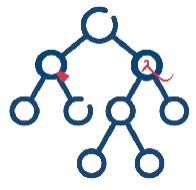
\includegraphics[height=1.0cm]{msca_logo.png}}%
    \end{center}

    \vspace{0.6cm}

    % Main title with Q logos on sides (with clickable links)
    \begin{center}
        \begin{minipage}{0.1\textwidth}
            \centering
            \href{https://quantlet.com}{
\includegraphics[height=1.1cm]{ql_logo.png}}
        \end{minipage}%
        \begin{minipage}{0.78\textwidth}
            \centering
            {\LARGE\bfseries\usebeamercolor[fg]{title}\inserttitle}

            \vspace{0.3cm}

            {\usebeamerfont{subtitle}\usebeamercolor[fg]{title}\insertsubtitle}
        \end{minipage}%
        \begin{minipage}{0.1\textwidth}
            \centering
            \href{https://quantinar.com}{
\includegraphics[height=1.1cm]{qr_logo.png}}
        \end{minipage}
    \end{center}

    \vspace{0.6cm}

    % Authors (left aligned)
    \hspace{0.5cm}{\usebeamerfont{author}\insertauthor}

    \vspace{0.3cm}

    % Institute/Affiliations (left aligned)
    \hspace{0.5cm}\begin{minipage}[t]{0.9\textwidth}
        \raggedright\small\insertinstitute
    \end{minipage}
}

%=============================================================================
% THEOREM ENVIRONMENTS
%=============================================================================
\theoremstyle{definition}
\setbeamertemplate{theorems}[numbered]
\ifdefined\tsalang
\newtheorem{defn}{Definiție}
\newtheorem{thm}{Teoremă}
\newtheorem{prop}{Propoziție}
\newtheorem{rmk}{Observație}
\else
\newtheorem{defn}{Definition}
\newtheorem{thm}{Theorem}
\newtheorem{prop}{Proposition}
\newtheorem{rmk}{Remark}
\fi

%=============================================================================
% CENTRED MINIPAGE (no extra vertical space)
%=============================================================================
\newenvironment{cminipage}[1]{%
    \par\noindent\hfill\begin{minipage}{#1}\ignorespaces
}{%
    \end{minipage}\hfill\null\par
}

%=============================================================================
% CUSTOM COMMANDS
%=============================================================================
\newcommand{\E}{\mathbb{E}}
\newcommand{\Var}{\text{Var}}
\newcommand{\Cov}{\text{Cov}}
\newcommand{\Corr}{\text{Corr}}
\newcommand{\R}{\mathbb{R}}
\newcommand{\N}{\mathbb{N}}
\newcommand{\Z}{\mathbb{Z}}
\newcommand{\B}{\mathbf{B}}
\newcommand{\imark}{\textcolor{MainBlue}{\textbullet}}
\newcommand{\RMSE}{\text{RMSE}}
\newcommand{\MAE}{\text{MAE}}
\newcommand{\MAPE}{\text{MAPE}}

% Boldface vector/matrix commands (VAR, VECM, state space; also used by the older TSA decks)
\newcommand{\bY}{\mathbf{Y}}
\newcommand{\bX}{\mathbf{X}}
\newcommand{\bA}{\mathbf{A}}
\newcommand{\bB}{\mathbf{B}}
\newcommand{\bepsilon}{\boldsymbol{\varepsilon}}
\newcommand{\bSigma}{\boldsymbol{\Sigma}}
\newcommand{\bPhi}{\boldsymbol{\Phi}}
\newcommand{\bGamma}{\boldsymbol{\Gamma}}
\newcommand{\bPi}{\boldsymbol{\Pi}}
\newcommand{\bc}{\mathbf{c}}
\newcommand{\balpha}{\boldsymbol{\alpha}}
\newcommand{\bbeta}{\boldsymbol{\beta}}
\newcommand{\bvarepsilon}{\boldsymbol{\varepsilon}}

% Legacy seminar marks (older TSA seminar decks)
\newcommand{\correct}{\textcolor{Forest}{\checkmark}}
\newcommand{\incorrect}{\textcolor{Crimson}{\texttimes}}
 se definește
%   \newcommand{\coursename}{Time Series Analysis}      (EN)
%   \newcommand{\coursename}{Serii de timp}       (RO)  și  \def\tsalang{ro}
% Fișierele .tex se află în EN/Courses, EN/Seminars, RO/Cursuri, RO/Seminarii (două niveluri sub rădăcină).
% Deck-urile sînt generate de latex/build_chapterN.py / build_seminarN.py (vezi latex/tsa_build.py).

\documentclass[9pt, aspectratio=169, t]{beamer}
\providecommand{\coursename}{Time Series Analysis}

% Ensure content fits on slides
\setbeamersize{text margin left=8mm, text margin right=8mm}
% Smaller institute font (title page)
\setbeamerfont{institute}{size=\footnotesize}

%=============================================================================
% THEME AND STYLE CONFIGURATION
%=============================================================================
\usetheme{default}
% Using default theme for clean header/footer control

% Color Palette (matching Redispatch PDF)
\definecolor{MainBlue}{RGB}{26, 58, 110}
\definecolor{AccentBlue}{RGB}{26, 58, 110}
\definecolor{IDAred}{RGB}{205, 0, 0}
\definecolor{DarkGray}{RGB}{51, 51, 51}
\definecolor{MediumGray}{RGB}{128, 128, 128}
\definecolor{LightGray}{RGB}{248, 248, 248}
\definecolor{VeryLightGray}{RGB}{235, 235, 235}
\definecolor{KeynoteGray}{RGB}{218, 218, 218}
\definecolor{SectionGray}{RGB}{120, 120, 120}
\definecolor{FooterGray}{RGB}{100, 100, 100}
\definecolor{Crimson}{RGB}{220, 53, 69}
\definecolor{Forest}{RGB}{46, 125, 50}
\definecolor{Amber}{RGB}{181, 133, 63}
\definecolor{Orange}{RGB}{230, 126, 34}
\definecolor{Purple}{RGB}{142, 68, 173}

% Gradient background (exact Keynote 315° gradient: white to RGB 218,218,218)
\setbeamertemplate{background}{%
    \begin{tikzpicture}[remember picture, overlay]
        \shade[shading=axis, shading angle=315,
        top color=white, bottom color=KeynoteGray]
        (current page.south west) rectangle (current page.north east);
    \end{tikzpicture}%
}
% Fallback solid color for compatibility
\setbeamercolor{background canvas}{bg=}

\setbeamercolor{palette primary}{bg=MainBlue, fg=white}
\setbeamercolor{palette secondary}{bg=MainBlue!85, fg=white}
\setbeamercolor{palette tertiary}{bg=MainBlue!70, fg=white}
\setbeamercolor{structure}{fg=MainBlue}
\setbeamercolor{title}{fg=IDAred}
\setbeamercolor{frametitle}{fg=IDAred, bg=}
\setbeamercolor{block title}{bg=MainBlue, fg=white}
\setbeamercolor{block body}{bg=VeryLightGray, fg=DarkGray}
\setbeamercolor{block title alerted}{bg=Crimson, fg=white}
\setbeamercolor{block body alerted}{bg=Crimson!8, fg=DarkGray}
\setbeamercolor{block title example}{bg=Forest, fg=white}
\setbeamercolor{block body example}{bg=Forest!8, fg=DarkGray}
\setbeamercolor{item}{fg=MainBlue}

% Footer colors (override Madrid theme blue)
\setbeamercolor{author in head/foot}{fg=FooterGray, bg=}
\setbeamercolor{title in head/foot}{fg=FooterGray, bg=}
\setbeamercolor{date in head/foot}{fg=FooterGray, bg=}
\setbeamercolor{section in head/foot}{fg=FooterGray, bg=}
\setbeamercolor{subsection in head/foot}{fg=FooterGray, bg=}

% Bullet styles (apply everywhere including blocks)
\setbeamertemplate{itemize item}{\color{MainBlue}$\boxdot$}
\setbeamertemplate{itemize subitem}{\color{MainBlue}$\blacktriangleright$}
\setbeamertemplate{itemize subsubitem}{\color{MainBlue}\tiny$\bullet$}
\setbeamertemplate{itemize/enumerate body begin}{\normalsize}
\setbeamertemplate{itemize/enumerate subbody begin}{\normalsize}

% Item spacing - compact style
\setlength{\leftmargini}{10pt}       % Level 1: minimal indent
\setlength{\leftmarginii}{10pt}      % Level 2: minimal additional indent
% Compact list spacing (zero extra space before/after lists in blocks)
\makeatletter
\def\@listi{\leftmargin\leftmargini \topsep 0pt \parsep 0pt \itemsep 0pt}
\def\@listii{\leftmargin\leftmarginii \topsep 0pt \parsep 0pt \itemsep 0pt}
\makeatother

\setbeamertemplate{navigation symbols}{}

%=============================================================================
% CUSTOM HEADLINE
%=============================================================================
\setbeamertemplate{headline}{%
    \vskip10pt%
    \hbox to \paperwidth{%
        \hskip0.5cm%
        {\small\color{FooterGray}\renewcommand{\hyperlink}[2]{##2}\insertsectionhead}%
        \hfill%
        \textcolor{FooterGray}{\small\insertframenumber}%
        \hskip0.5cm%
    }%
    \vskip4pt%
    {\color{FooterGray}\hrule height 0.4pt}%
}

%=============================================================================
% CUSTOM FOOTER
%=============================================================================
\usepackage{fontawesome5}

\setbeamertemplate{footline}{%
    {\color{FooterGray}\hrule height 0.4pt}%
    \vskip4pt%
    \hbox to \paperwidth{%
        \hskip0.5cm%
        \textcolor{FooterGray}{\small\coursename}%
        \hfill%
        \raisebox{-0.1em}{%
            \begin{tikzpicture}[x=0.08em, y=0.08em, line width=0.4pt]
                \draw[FooterGray] (0,3) -- (1,4) -- (2,3.5) -- (3,5) -- (4,4) -- (5,6) -- (6,5.5) -- (7,4) -- (8,5) -- (9,7) -- (10,6) -- (11,5) -- (12,6.5) -- (13,8) -- (14,7) -- (15,6) -- (16,7.5) -- (17,9) -- (18,8) -- (19,7) -- (20,8.5) -- (21,10) -- (22,9) -- (23,8) -- (24,9.5);
            \end{tikzpicture}%
        }%
        \hskip0.5cm%
    }%
    \vskip6pt%
}

%=============================================================================
% PACKAGES
%=============================================================================
\usepackage[utf8]{inputenc}
\DeclareUnicodeCharacter{03B1}{\ensuremath{\alpha}}
\usepackage[T1]{fontenc}
\usepackage{amsmath, amssymb, amsthm}
\usepackage{mathtools}
\usepackage{bm}
\usepackage{tikz}
\usetikzlibrary{arrows.meta, positioning, shapes, calc, decorations.pathreplacing, shadings}
\usepackage{booktabs}
\usepackage{multirow}
\usepackage{array}
\usepackage{graphicx}
\usepackage{animate}
\usepackage{hyperref}
\usepackage{colortbl}
\usepackage{listings}
\lstset{language=Python, basicstyle=\ttfamily\scriptsize, keywordstyle=\color{MainBlue}\bfseries,
  commentstyle=\color{Forest}, stringstyle=\color{Crimson}, breaklines=true,
  frame=none, backgroundcolor=\color{VeryLightGray}, xleftmargin=2mm}
\hypersetup{colorlinks=true, linkcolor=MainBlue, urlcolor=MainBlue}
\graphicspath{{../../logos/}{../../charts/}{../../photos/}}
\usepackage{xcolor}
\hfuzz=2pt  % Suppress tiny overfull warnings (<2pt)
\vfuzz=2pt  % Suppress tiny vertical overfull warnings (<2pt)
% \mathrm in the sans-serif family of the slides (beamer resets \mathrm to the serif family at \begin{document};
% this hook runs after beamer's, so WN, Var, RMSE, ... in formulas match the surrounding text)
% Bold vectors and matrices in the same sans-serif family: \mathbf{A} in sans bold (beamer's own \mathbf came out in
% medium weight), and the bold upright Greek capitals of \boldsymbol / \bm (\bSigma, \bPhi, \boldsymbol{\Theta}) in
% cmss bold: bm.sty fixes its "boldoperators" font when it is loaded (serif cmbx), before beamer switches the
% operators to cmss, so it is reset here.
\AtBeginDocument{%
  \SetMathAlphabet{\mathrm}{normal}{\encodingdefault}{\sfdefault}{\mddefault}{n}%
  \SetMathAlphabet{\mathrm}{bold}{\encodingdefault}{\sfdefault}{bx}{n}%
  \SetMathAlphabet{\mathbf}{normal}{\encodingdefault}{\sfdefault}{bx}{n}%
  \SetMathAlphabet{\mathbf}{bold}{\encodingdefault}{\sfdefault}{bx}{n}%
  \SetSymbolFont{boldoperators}{normal}{OT1}{cmss}{bx}{n}%
  \SetSymbolFont{boldoperators}{bold}{OT1}{cmss}{bx}{n}}

%=============================================================================
% QUANTLET COMMANDS
%   \quantlet{<displayed name>}{<url>}       (generic, compatible with the older TSA decks)
%   \tsaquantlet{Ch_05}{TSA_ch5_garch}       -> https://github.com/danpele/Time-Series-Analysis/tree/main/Quantlets/Ch_05/TSA_ch5_garch
%   \qlurl{<folder>} is defined per chapter by the generator (Quantlets/Ch_NN/<folder>)
%=============================================================================
\newcommand{\tsarepo}{https://github.com/danpele/Time-Series-Analysis}
\newcommand{\tsaqlbase}{https://github.com/danpele/Time-Series-Analysis/tree/main/Quantlets}
\newcommand{\quantlet}[2]{%
    \hfill\href{#2}{%
        \raisebox{-0.15em}{
\includegraphics[height=0.7em]{ql_logo.png}}%
        \textcolor{MainBlue}{\tiny\ #1}%
    }%
}
\newcommand{\tsaquantlet}[2]{\quantlet{\detokenize{#2}}{\tsaqlbase/#1/#2}}

%=============================================================================
% NOTEBOOKS (Google Colab)
%   \colaburl{notebooks/EN/chapter5_seminar_notebook.ipynb} -> the Colab link of a file in the TSA repo
%   \nb: the chapter notebook (each seminar deck redefines it with \renewcommand)
%=============================================================================
\newcommand{\colaburl}[1]{https://colab.research.google.com/github/danpele/Time-Series-Analysis/blob/main/#1}
\newcommand{\nb}{https://colab.research.google.com/github/danpele/Time-Series-Analysis/tree/main/notebooks/EN}
\newcommand{\nbname}{notebooks/EN}

%=============================================================================
% SLIDE HELPERS (used by the generators; the same as in MFM)
%=============================================================================
% local font size for list bodies (the preamble forces \normalsize)
\newcommand{\itemsize}[1]{\setbeamertemplate{itemize/enumerate body begin}{#1}\setbeamertemplate{itemize/enumerate subbody begin}{#1}}
\newcommand{\intitle}[1]{{\hypersetup{urlcolor=white}#1}}   % white links inside coloured title bars
\newcommand{\imgcap}[1]{{\scriptsize #1}\\[0.5mm]}          % caption under a photo
\newcommand{\imgcredit}[2]{{\tiny\color{FooterGray}\href{#1}{#2}}}   % image credit: source URL, author/licence
\newcommand{\aiprompt}[1]{{\ttfamily\color{MainBlue}#1}}     % a prompt to an AI assistant

%=============================================================================
% SEMINARS: student version by default; the instructor wrapper *_solutions.tex sets \solutionstrue
%=============================================================================
\makeatletter\@ifundefined{ifsolutions}{\expandafter\newif\csname ifsolutions\endcsname}{}\makeatother
\newcommand{\solonly}[1]{\ifsolutions #1\fi}
\newcommand{\propsub}{\ifsolutions\else\framesubtitle{\ifdefined\tsalang Rezolvarea se discută la seminar\else Solution discussed in class\fi}\fi}

%=============================================================================
% APPENDIX AND CHAPTER LINKS (latex/appendix_links.py writes the calls; it also re-declares these
% macros before \begin{document}, so the decks compile with or without this preamble block)
%=============================================================================
\providecommand{\tsaapplink}[3]{\hypertarget{#2}{}\hyperlink{#1}{\beamergotobutton{#3}}}
\providecommand{\tsaappback}[2]{\begin{tikzpicture}[remember picture,overlay]\node[anchor=south east] at ([xshift=-3mm,yshift=7mm]current page.south east){\hyperlink{#1}{\beamerreturnbutton{#2}}};\end{tikzpicture}}
\providecommand{\tsachlink}[2]{\href{#1}{#2}}
\providecommand{\tsachlinkt}[2]{\href{#1}{\usebeamercolor[fg]{frametitle}#2}}

%=============================================================================
% QUANTINAR COMMAND: link către un curs Quantinar (subiecte avansate)
%=============================================================================
\newcommand{\quantinar}[2]{%
    \href{#2}{%
        \raisebox{-0.15em}{
\includegraphics[height=0.8em]{qr_logo.png}}%
        \textcolor{MainBlue}{\scriptsize\ #1}%
    }%
}

%=============================================================================
% CUSTOM TITLE PAGE
%=============================================================================
\defbeamertemplate*{title page}{hybrid}[1][]
{
    \vspace{0.2cm}
    % Logos row - top header (with clickable links)
    \begin{center}
        \href{https://www.ase.ro}{
\includegraphics[height=1.0cm]{ase_logo.png}}\hspace{0.3cm}%
        \href{https://theida.net}{
\includegraphics[height=1.0cm]{ida_logo.png}}\hspace{0.3cm}%
        \href{https://blockchain-research-center.com}{
\includegraphics[height=1.0cm]{brc_logo.png}}\hspace{0.3cm}%
        \href{https://www.ai4efin.ase.ro}{
\includegraphics[height=1.0cm]{ai4efin_logo.png}}\hspace{0.3cm}%
        \href{https://ipe.ro/new}{
\includegraphics[height=1.0cm]{acad_logo.png}}\hspace{0.3cm}%
        \href{https://www.digital-finance-msca.com}{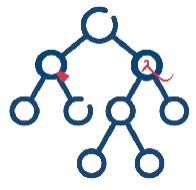
\includegraphics[height=1.0cm]{msca_logo.png}}%
    \end{center}

    \vspace{0.6cm}

    % Main title with Q logos on sides (with clickable links)
    \begin{center}
        \begin{minipage}{0.1\textwidth}
            \centering
            \href{https://quantlet.com}{
\includegraphics[height=1.1cm]{ql_logo.png}}
        \end{minipage}%
        \begin{minipage}{0.78\textwidth}
            \centering
            {\LARGE\bfseries\usebeamercolor[fg]{title}\inserttitle}

            \vspace{0.3cm}

            {\usebeamerfont{subtitle}\usebeamercolor[fg]{title}\insertsubtitle}
        \end{minipage}%
        \begin{minipage}{0.1\textwidth}
            \centering
            \href{https://quantinar.com}{
\includegraphics[height=1.1cm]{qr_logo.png}}
        \end{minipage}
    \end{center}

    \vspace{0.6cm}

    % Authors (left aligned)
    \hspace{0.5cm}{\usebeamerfont{author}\insertauthor}

    \vspace{0.3cm}

    % Institute/Affiliations (left aligned)
    \hspace{0.5cm}\begin{minipage}[t]{0.9\textwidth}
        \raggedright\small\insertinstitute
    \end{minipage}
}

%=============================================================================
% THEOREM ENVIRONMENTS
%=============================================================================
\theoremstyle{definition}
\setbeamertemplate{theorems}[numbered]
\ifdefined\tsalang
\newtheorem{defn}{Definiție}
\newtheorem{thm}{Teoremă}
\newtheorem{prop}{Propoziție}
\newtheorem{rmk}{Observație}
\else
\newtheorem{defn}{Definition}
\newtheorem{thm}{Theorem}
\newtheorem{prop}{Proposition}
\newtheorem{rmk}{Remark}
\fi

%=============================================================================
% CENTRED MINIPAGE (no extra vertical space)
%=============================================================================
\newenvironment{cminipage}[1]{%
    \par\noindent\hfill\begin{minipage}{#1}\ignorespaces
}{%
    \end{minipage}\hfill\null\par
}

%=============================================================================
% CUSTOM COMMANDS
%=============================================================================
\newcommand{\E}{\mathbb{E}}
\newcommand{\Var}{\text{Var}}
\newcommand{\Cov}{\text{Cov}}
\newcommand{\Corr}{\text{Corr}}
\newcommand{\R}{\mathbb{R}}
\newcommand{\N}{\mathbb{N}}
\newcommand{\Z}{\mathbb{Z}}
\newcommand{\B}{\mathbf{B}}
\newcommand{\imark}{\textcolor{MainBlue}{\textbullet}}
\newcommand{\RMSE}{\text{RMSE}}
\newcommand{\MAE}{\text{MAE}}
\newcommand{\MAPE}{\text{MAPE}}

% Boldface vector/matrix commands (VAR, VECM, state space; also used by the older TSA decks)
\newcommand{\bY}{\mathbf{Y}}
\newcommand{\bX}{\mathbf{X}}
\newcommand{\bA}{\mathbf{A}}
\newcommand{\bB}{\mathbf{B}}
\newcommand{\bepsilon}{\boldsymbol{\varepsilon}}
\newcommand{\bSigma}{\boldsymbol{\Sigma}}
\newcommand{\bPhi}{\boldsymbol{\Phi}}
\newcommand{\bGamma}{\boldsymbol{\Gamma}}
\newcommand{\bPi}{\boldsymbol{\Pi}}
\newcommand{\bc}{\mathbf{c}}
\newcommand{\balpha}{\boldsymbol{\alpha}}
\newcommand{\bbeta}{\boldsymbol{\beta}}
\newcommand{\bvarepsilon}{\boldsymbol{\varepsilon}}

% Legacy seminar marks (older TSA seminar decks)
\newcommand{\correct}{\textcolor{Forest}{\checkmark}}
\newcommand{\incorrect}{\textcolor{Crimson}{\texttimes}}


\newcommand{\qlurl}[1]{https://github.com/danpele/Time-Series-Analysis/tree/main/Quantlets/Ch_07/#1}
\renewcommand{\nb}{\colaburl{notebooks/EN/chapter7_seminar_notebook.ipynb}}
\renewcommand{\nbname}{chapter7\_seminar\_notebook.ipynb}
% left column: full width in the student version, narrower next to the solution
\newcommand{\taskw}{\ifsolutions 0.47\textwidth\else 0.96\textwidth\fi}
\newcommand{\solw}{\ifsolutions 0.49\textwidth\else 0pt\fi}

% Clickable citations (DOIs verified via Crossref)
\newcommand{\refHP}{\href{https://doi.org/10.1007/978-3-031-13584-2}{Huang și Petukhina (2022)}}
\newcommand{\refHamilton}{\href{https://doi.org/10.2307/j.ctv14jx6sm}{Hamilton (1994)}}
\newcommand{\refLut}{\href{https://doi.org/10.1007/978-3-540-27752-1}{Lütkepohl (2005)}}
\newcommand{\refJohBook}{\href{https://doi.org/10.1093/0198774508.001.0001}{Johansen (1995)}}
\newcommand{\refJus}{\href{https://doi.org/10.1093/oso/9780199285662.001.0001}{Juselius (2006)}}
\newcommand{\refEG}{\href{https://doi.org/10.2307/1913236}{Engle și Granger (1987)}}
\newcommand{\refGranger}{\href{https://doi.org/10.1016/0304-4076(81)90079-8}{Granger (1981)}}
\newcommand{\refGrangerN}{\href{https://doi.org/10.1257/0002828041464669}{Granger (2004)}}
\newcommand{\refGN}{\href{https://doi.org/10.1016/0304-4076(74)90034-7}{Granger și Newbold (1974)}}
\newcommand{\refMurray}{\href{https://doi.org/10.1080/00031305.1994.10476017}{Murray (1994)}}
\newcommand{\refPO}{\href{https://doi.org/10.2307/2938339}{Phillips și Ouliaris (1990)}}
\newcommand{\refMacKinnon}{\href{https://doi.org/10.1080/07350015.1994.10510005}{MacKinnon (1994)}}
\newcommand{\refMacKinnonb}{\href{https://ideas.repec.org/p/qed/wpaper/1227.html}{MacKinnon (2010)}}
\newcommand{\refSW}{\href{https://doi.org/10.1080/01621459.1988.10478707}{Stock și Watson (1988)}}
\newcommand{\refSWd}{\href{https://doi.org/10.2307/2951763}{Stock și Watson (1993)}}
\newcommand{\refDHSY}{\href{https://doi.org/10.2307/2231972}{Davidson et al.\ (1978)}}
\newcommand{\refBDM}{\href{https://doi.org/10.1111/1467-9892.00091}{Banerjee, Dolado și Mestre (1998)}}
\newcommand{\refJohA}{\href{https://doi.org/10.1016/0165-1889(88)90041-3}{Johansen (1988)}}
\newcommand{\refJohB}{\href{https://doi.org/10.2307/2938278}{Johansen (1991)}}
\newcommand{\refJJ}{\href{https://doi.org/10.1111/j.1468-0084.1990.mp52002003.x}{Johansen și Juselius (1990)}}
\newcommand{\refOL}{\href{https://doi.org/10.1111/j.1468-0084.1992.tb00013.x}{Osterwald-Lenum (1992)}}
\newcommand{\refMHM}{\href{https://doi.org/10.1002/(SICI)1099-1255(199909/10)14:5<563::AID-JAE530>3.0.CO;2-R}{MacKinnon, Haug și Michelis (1999)}}
\newcommand{\refRA}{\href{https://doi.org/10.1111/j.1467-9892.1992.tb00113.x}{Reinsel și Ahn (1992)}}
\newcommand{\refEY}{\href{https://doi.org/10.1016/0304-4076(87)90085-6}{Engle și Yoo (1987)}}
\newcommand{\refCD}{\href{https://doi.org/10.1080/07350015.1998.10524784}{Christoffersen și Diebold (1998)}}
\newcommand{\refCS}{\href{https://doi.org/10.1086/261502}{Campbell și Shiller (1987)}}
\newcommand{\refBalassa}{\href{https://doi.org/10.1086/258965}{Balassa (1964)}}
\newcommand{\refTT}{\href{https://doi.org/10.1257/0895330042632744}{Taylor și Taylor (2004)}}
\newcommand{\refGGR}{\href{https://doi.org/10.1093/rfs/hhj020}{Gatev, Goetzmann și Rouwenhorst (2006)}}
\newcommand{\refDoFaff}{\href{https://doi.org/10.2469/faj.v66.n4.1}{Do și Faff (2010)}}

\title[Serii de timp]{Serii de timp}
\subtitle{Seminarul 7: Cointegrare și VECM\ifsolutions\ (versiunea profesorului)\fi}
\author[D.T. Pele]{Daniel Traian PELE}
\institute{Academia de Studii Economice din București\\
IDA Institute Digital Assets\\
Blockchain Research Center\\
AI4EFin Artificial Intelligence for Energy Finance\\
Academia Română, Institutul de Prognoză Economică\\
MSCA Digital Finance}
\date{}

%=============================================================================
\providecommand{\tsaapplink}[3]{\hypertarget{#2}{}\hyperlink{#1}{\beamergotobutton{#3}}}  % APPLINKS-MACROS
\providecommand{\tsaappback}[2]{\begin{tikzpicture}[remember picture,overlay]\node[anchor=south east] at ([xshift=-3mm,yshift=7mm]current page.south east){\hyperlink{#1}{\beamerreturnbutton{#2}}};\end{tikzpicture}}  % APPLINKS-MACROS
\providecommand{\tsachlink}[2]{\href{#1}{#2}}  % APPLINKS-MACROS
\providecommand{\tsachlinkt}[2]{\href{#1}{\usebeamercolor[fg]{frametitle}#2}}  % APPLINKS-MACROS
\begin{document}
%=============================================================================

{
\setbeamertemplate{headline}{}
\setbeamertemplate{footline}{}
\begin{frame}[noframenumbering]
    \titlepage
\end{frame}
}
% BEGIN-ACRONYMS (generat de latex/acronyms.py; nu editati manual)
\begin{frame}{Acronime folosite în acest material}
\setbeamertemplate{itemize/enumerate body begin}{\tiny}
\begin{columns}[T]
\begin{column}{0.49\textwidth}
\begin{itemize}\setlength{\itemsep}{0pt}
    \item \textbf{ADF}: Augmented Dickey–Fuller (test) — testul Dickey–Fuller augmentat
    \item \textbf{AI}: Artificial Intelligence (inteligență artificială)
    \item \textbf{BIC}: Bayesian Information Criterion (criteriul informațional bayesian (Schwarz))
    \item \textbf{BNR}: Banca Națională a României
    \item \textbf{BVB}: Bursa de Valori București
    \item \textbf{ECM}: Error Correction Model (model cu corecția erorii)
    \item \textbf{EODHD}: EOD Historical Data (market-data provider) — furnizor de date de piață
    \item \textbf{FRED}: Federal Reserve Economic Data (baza de date economice a Rezervei Federale din St. Louis)
    \item \textbf{GS1}: 1-year Treasury constant-maturity yield (FRED series code) — codul FRED al randamentului titlurilor de stat americane la 1 an
    \item \textbf{GS10}: 10-year Treasury constant-maturity yield (FRED series code) — codul FRED al randamentului titlurilor de stat americane la 10 ani
    \item \textbf{HUF}: Hungarian forint (ISO 4217 code) — forintul maghiar (codul ISO 4217)
    \item \textbf{OLS}: Ordinary Least Squares (metoda celor mai mici pătrate)
    \item \textbf{PIB}: Produsul intern brut
\end{itemize}
\end{column}
\begin{column}{0.49\textwidth}
\begin{itemize}\setlength{\itemsep}{0pt}
    \item \textbf{PLN}: Polish zloty (ISO 4217 code) — zlotul polonez (codul ISO 4217)
    \item \textbf{ROBOR}: Romanian Interbank Offer Rate (rata dobînzii la care băncile din România oferă depozite interbancare)
    \item \textbf{SUA}: Statele Unite ale Americii
    \item \textbf{VAR}: Vector AutoRegression (model vector autoregresiv)
    \item \textbf{VECM}: Vector Error Correction Model (model vectorial cu corecția erorii)
\end{itemize}
\end{column}
\end{columns}
\end{frame}
% END-ACRONYMS

\begin{frame}{Întrebarea de azi și traseul}
\itemsize{\small}
\begin{itemize}
    \item \textbf{Întrebarea}: sînt două sau mai multe serii $I(1)$ legate printr-un echilibru pe termen lung, cît de repede revin la el și cine face ajustarea?
    \begin{itemize}
        \item seminarul are loc \textbf{înaintea} Cursului 7: secțiunea „Noțiuni necesare azi” dă toate definițiile folosite în cerințe
    \end{itemize}
    \item Traseul
    \begin{itemize}
        \item Partea A: statistici Engle--Granger calculate de mînă; un ECM și timpul lui de înjumătățire; un VECM cu două variabile; statistici Johansen; de la VAR la VECM
        \item Partea B: ratele dobînzii din SUA; consumul și PIB-ul României; EUR/RON, EUR/HUF și EUR/PLN; ROBOR, randamentul la 10 ani al României și Euribor
        \item Partea C: pairs trading pe două bănci din România și un răspuns AI de verificat
    \end{itemize}
    \item Notebook-ul de azi: \href{\nb}{deschideți notebook-ul seminarului în Google Colab}; fiecare cerință indică secțiunea din notebook
\end{itemize}
\end{frame}

\begin{frame}{Harta exercițiilor}
\itemsize{\small}
\begin{center}
\footnotesize
\begin{tabular}{>{\raggedright\arraybackslash}p{1.1cm}>{\raggedright\arraybackslash}p{7.5cm}>{\raggedright\arraybackslash}p{1.9cm}>{\raggedright\arraybackslash}p{1.4cm}}
\toprule
\textbf{Cerința} & \textbf{Întrebarea} & \textbf{Tipul} & \textbf{Model} \\
\midrule
A1, A2 & o statistică Engle--Granger cu două și cu trei variabile & Rezolvat, Propus & A1 \\
A3, A4 & un ECM și un VECM cu două variabile: viteză și timp de înjumătățire & Rezolvat, Propus & A3 \\
A5, A6 & statistici Johansen din valori proprii; un VAR(2) scris ca VECM & Rezolvat, Propus & A5 \\
B1, B2 & Engle--Granger și ECM: randamentele din SUA; consumul și PIB-ul României & Rezolvat, Propus & B1 \\
B3, B4 & Johansen și VECM: trei monede; trei rate ale dobînzii & Rezolvat, Propus & B3 \\
C1, C2 & pairs trading în afara eșantionului; ce este greșit într-un răspuns AI? & Propus & B1, B3 \\
\bottomrule
\end{tabular}
\end{center}
\begin{itemize}
    \item \textbf{[Rezolvat]}: rezolvarea completă în slide-uri și în notebook, un model de urmat; \textbf{[Propus]}: îl rezolvați dumneavoastră, după model
\end{itemize}
\end{frame}

\begin{frame}{Datele folosite}
\itemsize{\small}
\begin{center}
\footnotesize
\begin{tabular}{llll}
\toprule
\textbf{Seria} & \textbf{Sursa} & \textbf{Frecvența} & \textbf{Perioada} \\
\midrule
Randamentele titlurilor de stat SUA, 1 și 10 ani & FRED (GS1, GS10) & lunar & 1960--2026 \\
Consumul gospodăriilor și PIB-ul, România & Eurostat (namq\_10\_gdp) & trimestrial, ajustat sezonier & 1995--2026 \\
EUR/RON, EUR/HUF, EUR/PLN & cursurile de referință BNR & sfîrșitul lunii & 2005--2026 \\
ROBOR 3M, Euribor 3M & Eurostat (irt\_st\_m) & lunar & 2010--2026 \\
Randamentul la 10 ani, România & EODHD & zilnic, media lunară & 2010--2026 \\
Banca Transilvania, BRD & EODHD & zilnic, închidere ajustată & 2014--2026 \\
\bottomrule
\end{tabular}
\end{center}
\begin{itemize}
    \item Nivelurile ca $100\ln$ (consum, PIB, cursuri, prețuri ale acțiunilor); ratele dobînzii în \% pe an
    \item În notebook: \texttt{adf\_test}, \texttt{eg\_test} (Engle--Granger și Phillips--Ouliaris), \texttt{ecm\_fit}, \texttt{johansen}; nu este nevoie de cont sau de cheie
\end{itemize}
\end{frame}


%=============================================================================
\section{Noțiuni necesare azi}
%=============================================================================

\begin{frame}{Noțiuni necesare azi (1/4): cointegrarea}
\itemsize{\small}
\begin{itemize}
    \item $y_t \sim I(1)$: $y_t$ are o rădăcină unitară, iar $\Delta y_t = y_t - y_{t-1}$ este staționar (\tsachlink{https://danpele.github.io/Time-Series-Analysis/RO/Cursuri/capitol3_radacini_unitare_modele_arima.pdf}{Capitolul 3}; testul ADF, $H_0$: rădăcină unitară)
    \begin{itemize}
        \item regresia unei serii $I(1)$ pe o alta, fără legătură cu ea, este o \textbf{regresie falsă}: $t$ mare, $R^2$ mare
    \end{itemize}
    \item \textbf{Cointegrarea}: serii $I(1)$ $y_{1t}, \dots, y_{nt}$ pentru care o combinație $\beta^\top\mathbf y_t$ este staționară
    \begin{itemize}
        \item $\beta$: vectorul de cointegrare, normalizat cu un coeficient egal cu 1; $u_t = \beta^\top\mathbf y_t - \mu$: eroarea de echilibru
        \item seriile au trenduri stochastice comune: $n$ variabile, $r$ vectori de cointegrare, $n - r$ trenduri comune
    \end{itemize}
    \item Exemplu: rata dobînzii la 1 an și cea la 10 ani rătăcesc, dar diferența dintre ele rămîne într-o bandă
\end{itemize}
\end{frame}

\begin{frame}{Noțiuni necesare azi (2/4): testul Engle--Granger}
\itemsize{\small}
\begin{itemize}
    \item \textbf{Pasul 1}: OLS în niveluri, $y_t = a + b x_t + u_t$; reziduurile $\hat u_t$
    \begin{itemize}
        \item \textbf{Pasul 2}: ADF pe $\hat u_t$ fără constantă: $\Delta\hat u_t = \gamma\hat u_{t-1} + \sum_j\delta_j\Delta\hat u_{t-j} + e_t$, $\tau = \hat\gamma/\mathrm{SE}(\hat\gamma)$
        \item $H_0$: fără cointegrare ($\gamma = 0$); respingem dacă $\tau$ este sub valoarea critică
    \end{itemize}
    \item \textbf{Valorile critice} (MacKinnon, cu constantă, $T$ mare): mai negative decît cele Dickey--Fuller, deoarece OLS face ca $\hat u_t$ să pară staționar
    \begin{itemize}
        \item 5\%: $-2{,}86$ (o serie, Dickey--Fuller); $-3{,}34$ (2 variabile); $-3{,}74$ (3 variabile)
    \end{itemize}
    \item \textbf{Phillips--Ouliaris} $Z_t$: aceeași $H_0$ și aceleași valori critice; fără decalaje, cu o corecție prin varianța pe termen lung
    \begin{itemize}
        \item în Python: \texttt{coint} (\texttt{statsmodels}), \texttt{phillips\_ouliaris} (\texttt{arch})
    \end{itemize}
\end{itemize}
\end{frame}

\begin{frame}{Noțiuni necesare azi (3/4): corecția erorii}
\itemsize{\small}
\begin{itemize}
    \item \textbf{ECM} (error correction model, modelul cu corecția erorii): $\Delta y_t = c + \gamma\,\hat u_{t-1} + \delta_0\,\Delta x_t + \dots + \varepsilon_t$, cu $\hat u_{t-1} = y_{t-1} - \hat a - \hat b x_{t-1}$
    \begin{itemize}
        \item $\gamma < 0$: \textbf{viteza de ajustare}, fracțiunea din distanța din perioada anterioară închisă de $y$; $\delta_0$: efectul pe termen scurt; $b$: efectul pe termen lung
    \end{itemize}
    \item \textbf{Timpul de înjumătățire}: o distanță scade ca $(1 + \gamma)^h$; jumătate din ea dispare după $h_{1/2} = \ln 0{,}5/\ln(1 + \gamma)$ perioade
    \begin{itemize}
        \item exemplu: $\gamma = -0{,}5$ dă $h_{1/2} = 1$; $\gamma = -0{,}1$ dă circa 6{,}6 perioade
    \end{itemize}
    \item Toți termenii unui ECM sînt staționari: OLS și testele $t$ sînt valide
\end{itemize}
\end{frame}

\begin{frame}{Noțiuni necesare azi (4/4): VECM și Johansen}
\itemsize{\small}
\begin{itemize}
    \item \textbf{VECM}: $\Delta\mathbf y_t = \Pi\mathbf y_{t-1} + \sum_{i=1}^{p-1}\Gamma_i\Delta\mathbf y_{t-i} + \mathbf u_t$; dintr-un VAR($p$) (\tsachlink{https://danpele.github.io/Time-Series-Analysis/RO/Cursuri/capitol6_modele_var_cauzalitate_granger.pdf}{Capitolul 6}): $\Pi = A_1 + \dots + A_p - I$, $\Gamma_i = -(A_{i+1} + \dots + A_p)$
    \begin{itemize}
        \item $r = \mathrm{rang}(\Pi)$: 0 = fără cointegrare; $0 < r < n$: $\Pi = \alpha\beta^\top$, $r$ vectori de cointegrare (coloanele lui $\beta$) și coeficienții de ajustare $\alpha$
        \item $\alpha_i = 0$: $y_i$ nu se ajustează (\textbf{slab exogenă})
    \end{itemize}
    \item \textbf{Johansen}: valorile proprii $\hat\lambda_1 \ge \dots \ge \hat\lambda_n$; urma $= -T\sum_{i>r}\ln(1 - \hat\lambda_i)$, valoarea proprie maximă $= -T\ln(1 - \hat\lambda_{r+1})$
    \begin{itemize}
        \item testăm $r = 0$, $r \le 1$ etc.: rangul este primul $r$ nerespins; valori critice de 5\% cu constantă, $n = 3$: urma 29{,}80; 15{,}49; 3{,}84; valoarea maximă 21{,}13; 14{,}26; 3{,}84
    \end{itemize}
\end{itemize}
\end{frame}


%=============================================================================
\section{Partea A: calcule pe hîrtie}
%=============================================================================

\begin{frame}{A1: o statistică Engle--Granger [Rezolvat]}
\itemsize{\scriptsize}
\begin{columns}[T]
\begin{column}{0.47\textwidth}
\begin{block}{Cerință}
\begin{itemize}
    \item Două serii $I(1)$, $T = 200$. Pasul 1 dă reziduurile $\hat u_t$; pasul 2 dă $\Delta\hat u_t = -0{,}118\,\hat u_{t-1}$, cu $\mathrm{SE} = 0{,}036$.
    \item 1. Calculați $\tau$.
    \item 2. Comparați $\tau$ cu valorile Engle--Granger de 5\% și 10\% pentru 2 variabile, $-3{,}37$ și $-3{,}07$, și decideți.
    \item 3. Precizați ce ar fi concluzionat valoarea Dickey--Fuller $-2{,}88$.
    \item 4. Explicați de ce diferă cele două valori critice.
    \item Raportați: o valoare, două decizii și o frază.
\end{itemize}
\end{block}
\end{column}
\begin{column}{0.49\textwidth}
\begin{exampleblock}{Rezolvare}
\begin{itemize}
    \item 1. $\tau = -0{,}118/0{,}036 = -3{,}28$
    \item 2. $-3{,}28 > -3{,}37$: nu respingem „fără cointegrare” la 5\% (p = 0{,}058); $-3{,}28 < -3{,}07$: respingem la 10\%
    \item 3. $-3{,}28 < -2{,}88$: tabelul Dickey--Fuller ar raporta greșit cointegrare la 5\%
    \item 4. OLS alege $\hat b$ astfel încît să minimizeze varianța reziduurilor, deci $\hat u_t$ pare mai staționar decît o eroare adevărată: distribuția din ipoteza nulă se deplasează la stînga.
\end{itemize}
\end{exampleblock}
\end{column}
\end{columns}
\end{frame}

\begin{frame}{A2: trei variabile [Propus]}
\propsub
\itemsize{\scriptsize}
\begin{columns}[T]
\begin{column}{\taskw}
\begin{block}{Cerință}
\begin{itemize}
    \item Trei serii $I(1)$, $T = 150$: $y_t$ regresat pe $x_{1t}$ și $x_{2t}$. Pasul 2 dă $\hat\gamma = -0{,}162$, $\mathrm{SE} = 0{,}041$. Model: A1.
    \item 1. Calculați $\tau$.
    \item 2. Decideți la 5\% și la 1\% cu valorile pentru 3 variabile, $-3{,}80$ și $-4{,}39$.
    \item 3. Precizați ce valoare critică ar folosi greșit un student care ar uita de $x_{2t}$ (2 variabile: $-3{,}38$).
    \item 4. Precizați cîți vectori de cointegrare poate găsi metoda Engle--Granger cu trei variabile.
    \item Raportați: o valoare, două decizii și două fraze.
\end{itemize}
\end{block}
\end{column}
\begin{column}{\solw}
\solonly{%
\begin{exampleblock}{Rezolvare}
\begin{itemize}
    \item 1. $\tau = -0{,}162/0{,}041 = -3{,}95$
    \item 2. $-3{,}95 < -3{,}80$: respingem la 5\% (p = 0{,}028); $-3{,}95 > -4{,}39$: nu și la 1\%
    \item 3. $-3{,}38$: mai puțin negativă decît valoarea corectă; aici decizia ar fi aceeași, dar în general testul ar respinge prea des
    \item 4. Unul: reziduurile unei singure regresii; cu trei variabile pot exista doi vectori, pe care doar metoda Johansen îi poate găsi.
\end{itemize}
\end{exampleblock}
}
\end{column}
\end{columns}
\end{frame}

\begin{frame}{A3: un model cu corecția erorii [Rezolvat]}
\itemsize{\scriptsize}
\begin{columns}[T]
\begin{column}{0.47\textwidth}
\begin{block}{Cerință}
\begin{itemize}
    \item ECM estimat (logaritmul consumului $c_t$ și al venitului $y_t$, în \%): $\Delta c_t = 0{,}2 + 0{,}5\,\Delta y_t - 0{,}25\,(c_{t-1} - 0{,}9\,y_{t-1})$.
    \item 1. Precizați efectul pe termen lung și efectul pe termen scurt al venitului asupra consumului.
    \item 2. Interpretați coeficientul $-0{,}25$ și calculați timpul de înjumătățire.
    \item 3. Calculați $\Delta c_t$ dacă $c_{t-1} - 0{,}9\,y_{t-1} = 2$ și $\Delta y_t = 1$.
    \item 4. Precizați ce ar însemna un coeficient de $+0{,}25$.
    \item Raportați: două elasticități, un timp de înjumătățire, o prognoză și o frază.
\end{itemize}
\end{block}
\end{column}
\begin{column}{0.49\textwidth}
\begin{exampleblock}{Rezolvare}
\begin{itemize}
    \item 1. Termen lung: 0,9 (din echilibrul $c = 0{,}9y$ + const.); termen scurt: 0,5 (în aceeași perioadă)
    \item 2. Un sfert din distanța din perioada anterioară se închide în fiecare perioadă; $h_{1/2} = \ln 0{,}5/\ln 0{,}75 = 2{,}41$ perioade
    \item 3. $\Delta c_t = 0{,}2 + 0{,}5 \cdot 1 - 0{,}25 \cdot 2 = 0{,}2$: corecția erorii anulează efectul pe termen scurt
    \item 4. Consumul s-ar îndepărta de echilibru după o abatere: fără corecția erorii, fără cointegrare.
\end{itemize}
\end{exampleblock}
\end{column}
\end{columns}
\end{frame}

\begin{frame}{A4: un VECM cu două variabile [Propus]}
\propsub
\itemsize{\scriptsize}
\begin{columns}[T]
\begin{column}{\taskw}
\begin{block}{Cerință}
\begin{itemize}
    \item $\Delta y_{1t} = -0{,}20\,z_{t-1} + u_{1t}$, $\Delta y_{2t} = 0{,}05\,z_{t-1} + u_{2t}$, cu $z_t = y_{1t} - y_{2t}$. Model: A3.
    \item 1. Scrieți $\alpha$, $\beta$ și $\Pi = \alpha\beta^\top$ și precizați rangul lui $\Pi$.
    \item 2. Explicați care variabilă face cea mai mare parte a ajustării.
    \item 3. Arătați că $z_t = (1 + \beta^\top\alpha)\,z_{t-1} + (u_{1t} - u_{2t})$ și calculați timpul de înjumătățire.
    \item Raportați: o matrice, un rang, un timp de înjumătățire și o frază.
\end{itemize}
\end{block}
\end{column}
\begin{column}{\solw}
\solonly{%
\begin{exampleblock}{Rezolvare}
\begin{itemize}
    \item 1. $\alpha = (-0{,}20; 0{,}05)^\top$, $\beta = (1, -1)^\top$; $\Pi = \begin{pmatrix} -0{,}20 & 0{,}20 \\ 0{,}05 & -0{,}05 \end{pmatrix}$, $\det\Pi = 0$, rangul 1
    \item 2. $y_1$: închide 20\% din distanță pe perioadă, $y_2$ doar 5\%; $y_2$ este aproape slab exogenă
    \item 3. $\Delta z_t = \Delta y_{1t} - \Delta y_{2t} = (-0{,}20 - 0{,}05)\,z_{t-1} + \dots$; $\beta^\top\alpha = -0{,}25$, $z_t = 0{,}75\,z_{t-1} + \dots$; timpul de înjumătățire 2{,}41 perioade
\end{itemize}
\end{exampleblock}
}
\end{column}
\end{columns}
\end{frame}

\begin{frame}{A5: statistici Johansen din valori proprii [Rezolvat]}
\itemsize{\scriptsize}
\begin{columns}[T]
\begin{column}{0.47\textwidth}
\begin{block}{Cerință}
\begin{itemize}
    \item Trei serii $I(1)$, $T = 200$, cazul cu constantă; valorile proprii Johansen sînt 0,120; 0,045 și 0,008.
    \item 1. Calculați statisticile urmei pentru $r = 0$, $r \le 1$ și $r \le 2$.
    \item 2. Calculați statisticile valorii proprii maxime.
    \item 3. Comparați cu valorile de 5\% (urma $29{,}80$; $15{,}49$; $3{,}84$; maxima $21{,}13$; $14{,}26$; $3{,}84$) și alegeți rangul.
    \item 4. Precizați numărul trendurilor comune.
    \item Raportați: șase statistici, un rang și un număr de trenduri.
\end{itemize}
\end{block}
\end{column}
\begin{column}{0.49\textwidth}
\begin{exampleblock}{Rezolvare}
\begin{itemize}
    \item 1. $-200[\ln 0{,}880 + \ln 0{,}955 + \ln 0{,}992] = 36{,}38$; $-200[\ln 0{,}955 + \ln 0{,}992] = 10{,}82$; $-200\ln 0{,}992 = 1{,}61$
    \item 2. 25{,}57; 9{,}21; 1{,}61
    \item 3. $r = 0$ respins de ambele teste ($36{,}38 > 29{,}80$, $25{,}57 > 21{,}13$); $r \le 1$ nerespins: rangul 1
    \item 4. $n - r = 3 - 1 = 2$ trenduri stochastice comune.
\end{itemize}
\end{exampleblock}
\end{column}
\end{columns}
\end{frame}

\begin{frame}{A6: de la VAR(2) la VECM [Propus]}
\propsub
\itemsize{\scriptsize}
\begin{columns}[T]
\begin{column}{\taskw}
\begin{block}{Cerință}
\begin{itemize}
    \item $\mathbf y_t = A_1\mathbf y_{t-1} + A_2\mathbf y_{t-2} + \mathbf u_t$ cu $A_1 = \begin{pmatrix} 0{,}7 & 0{,}2 \\ 0{,}1 & 0{,}7 \end{pmatrix}$, $A_2 = \begin{pmatrix} 0{,}1 & 0 \\ 0 & 0{,}2 \end{pmatrix}$. Model: A5.
    \item 1. Calculați $\Pi = A_1 + A_2 - I$ și $\Gamma_1 = -A_2$.
    \item 2. Arătați că $\Pi$ are rangul 1 și scrieți-o ca $\alpha\beta^\top$, cu $\beta = (1, -1)^\top$.
    \item 3. Interpretați semnele lui $\alpha$.
    \item Raportați: două matrice, $\alpha$ și o frază.
\end{itemize}
\end{block}
\end{column}
\begin{column}{\solw}
\solonly{%
\begin{exampleblock}{Rezolvare}
\begin{itemize}
    \item 1. $\Pi = \begin{pmatrix} -0{,}2 & 0{,}2 \\ 0{,}1 & -0{,}1 \end{pmatrix}$, $\Gamma_1 = \begin{pmatrix} -0{,}1 & 0 \\ 0 & -0{,}2 \end{pmatrix}$
    \item 2. $\det\Pi = 0{,}02 - 0{,}02 = 0$, rînduri proporționale: rangul 1; $\alpha = (-0{,}2; 0{,}1)^\top$; verificare: VAR-ul are o rădăcină egală cu 1 (celelalte 1{,}34; 4{,}42; 8{,}42)
    \item 3. Cînd $y_1 > y_2$: $y_1$ scade, iar $y_2$ crește: ambele corectează distanța; $\beta^\top\alpha = -0{,}3$, timp de înjumătățire de circa 1{,}9 perioade.
\end{itemize}
\end{exampleblock}
}
\end{column}
\end{columns}
\end{frame}


%=============================================================================
\section{Partea B: date reale și interpretare}
%=============================================================================

\begin{frame}{B1: randamentele din SUA la 1 an și la 10 ani [Rezolvat]}
\itemsize{\footnotesize}
\begin{itemize}
\item \textbf{Întrebarea}: sînt cointegrate randamentele titlurilor de stat la 1 an și la 10 ani, cît de repede se închide distanța dintre ele și care rată o închide?
\item \textbf{Date}: FRED GS1 și GS10, medii lunare, \% pe an, ianuarie 1960--septembrie 2026
\item \textbf{Cerințe}
\begin{enumerate}
    \item Aplicați ADF (cu constantă) pe ambele randamente și pe variația randamentului la 10 ani.
    \item Aplicați Engle--Granger (10 ani pe 1 an) și Phillips--Ouliaris și comparați cu valoarea Engle--Granger de 5\%.
    \item Estimați ECM pentru randamentul la 10 ani (cîte un decalaj din fiecare diferență) și aceeași ecuație pentru randamentul la 1 an.
    \item Interpretare: dacă randamentul la 10 ani este cu 1 punct procentual peste echilibru, cît timp trece pînă se închide jumătate din distanță și prin care rată?
\end{enumerate}
\item \textbf{Raportați}: trei valori p ADF, două teste de cointegrare, doi coeficienți de ajustare și o frază
\item Notebook: secțiunea B1
\end{itemize}
\end{frame}

\begin{frame}{B1: rezolvare [Rezolvat]}
\itemsize{\scriptsize}
\begin{center}
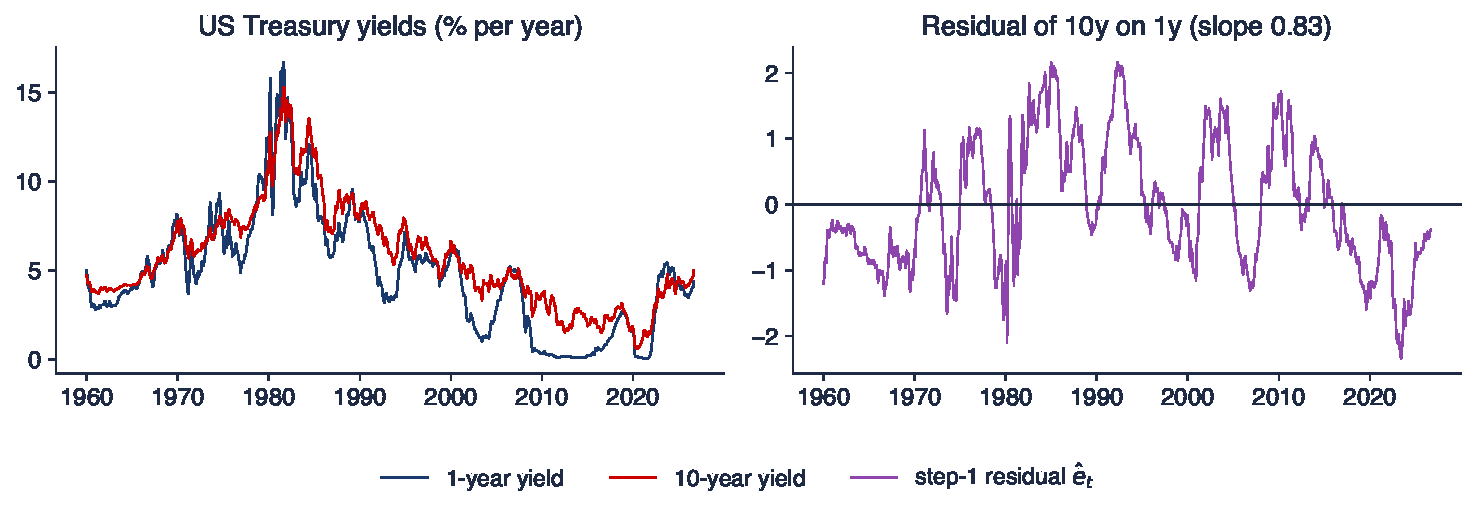
\includegraphics[width=0.96\textwidth,height=0.34\textheight,keepaspectratio]{ch7_sem_b1.pdf}
\end{center}
\vspace{-2mm}
\begin{itemize}
    \item ADF p = 0{,}26 (1 an), 0{,}63 (10 ani): rădăcini unitare; variația: p $<$\,0{,}001; ambele randamente sînt $I(1)$
    \item Pasul 1: $\hat\imath^{(10)}_t = 1{,}76 + 0{,}827\,i^{(1)}_t$; pasul 2: $\tau = -3{,}59$ (19 decalaje) $< -3{,}34$: cointegrare la 5\% (p = 0{,}025); Phillips--Ouliaris $Z_t = -3{,}65$ (p = 0{,}022)
    \item ECM, 10 ani: $\hat\gamma = -0{,}0295$ ($t = -4{,}81$), $\hat\delta_0 = 0{,}53$; 1 an: $\hat\gamma = 0{,}0172$ ($t = 1{,}25$), nesemnificativ
    \item Interpretare: timpul de înjumătățire $\ln 0{,}5/\ln(1 -0{,}0295) = 23{,}1$ luni, circa doi ani; randamentul la 10 ani închide distanța, iar cel la 1 an (stabilit de politica monetară) nu reacționează
\end{itemize}\quantlet{TSA\_ch7\_seminar}{\qlurl{TSA_ch7_seminar}}
\end{frame}

\begin{frame}{B2: consumul și PIB-ul în România [Propus]}
\itemsize{\footnotesize}
\begin{itemize}
\item \textbf{Întrebarea}: este consumul gospodăriilor din România cointegrat cu PIB-ul, cum sugerează „marile rapoarte”?
\item \textbf{Date}: Eurostat, consumul real al gospodăriilor și PIB-ul real, volume înlănțuite, ajustate sezonier, 1995--2026; $c_t$, $y_t$ ca $100\ln$; model: B1
\item \textbf{Cerințe}
\begin{enumerate}
    \item Aplicați ADF (constantă și trend) pe $c_t$ și $y_t$ și ADF (constantă) pe variațiile lor.
    \item Aplicați Engle--Granger ($c_t$ pe $y_t$) și Phillips--Ouliaris și raportați panta.
    \item Reprezentați grafic raportul dintre consum și PIB și aplicați ADF pe $c_t - y_t$.
    \item Interpretare: are sens o pondere stabilă a consumului pentru România în perioada 1995--2026?
\end{enumerate}
\item \textbf{Raportați}: patru teste ADF, două teste de cointegrare, un grafic și două fraze
\item Notebook: secțiunea B2
\end{itemize}
\end{frame}

\ifsolutions
\begin{frame}{B2: rezolvare [Propus]}
\itemsize{\scriptsize}
\begin{center}
\includegraphics[width=0.96\textwidth,height=0.34\textheight,keepaspectratio]{ch7_sem_b2.pdf}
\end{center}
\vspace{-2mm}
\begin{itemize}
    \item ADF p = 0{,}37 ($c_t$), 0{,}20 ($y_t$); variațiile: p $<$\,0{,}001 și $<$\,0{,}001: ambele $I(1)$ ($T = 126$)
    \item Panta 1{,}46; Engle--Granger $\tau = -2{,}32$ (8 decalaje), p = 0{,}36: fără cointegrare; Phillips--Ouliaris $Z_t = -6{,}80$, p $<$\,0{,}001: cointegrare; testele nu concordă
    \item $c_t - y_t$: ADF p = 0{,}46; ponderea a crescut de la circa 46\% la 73\% (raport de volume înlănțuite, o măsură aproximativă)
    \item Interpretare: nu; o economie în convergență, cu credit și remitențe în creștere, a mărit consumul mai repede decît PIB-ul; o pantă de 1{,}46 nu este un „mare raport”, iar verdictul depinde de numărul de decalaje
\end{itemize}\quantlet{TSA\_ch7\_seminar}{\qlurl{TSA_ch7_seminar}}
\end{frame}
\fi

\begin{frame}{B3: trei monede central-europene [Rezolvat]}
\itemsize{\footnotesize}
\begin{itemize}
\item \textbf{Întrebarea}: au EUR/RON, EUR/HUF și EUR/PLN un echilibru comun pe termen lung?
\item \textbf{Date}: cursurile de referință BNR (cursuri încrucișate pentru HUF și PLN), la sfîrșitul lunii, $100\ln$, din iulie 2005
\item \textbf{Cerințe}
\begin{enumerate}
    \item Aplicați ADF pe fiecare curs.
    \item Aplicați testele Johansen ale urmei și ale valorii proprii maxime, cu constantă și decalaje după BIC.
    \item Comparați cu cele trei teste Engle--Granger pe perechi și cu corelațiile nivelurilor și ale variațiilor.
    \item Interpretare: ar trebui modelate cele trei cursuri cu un VECM?
\end{enumerate}
\item \textbf{Raportați}: trei valori p ADF, un tabel cu șase statistici Johansen, un rang și o frază
\item Notebook: secțiunea B3
\end{itemize}
\end{frame}

\begin{frame}{B3: rezolvare [Rezolvat]}
\itemsize{\scriptsize}
\begin{center}
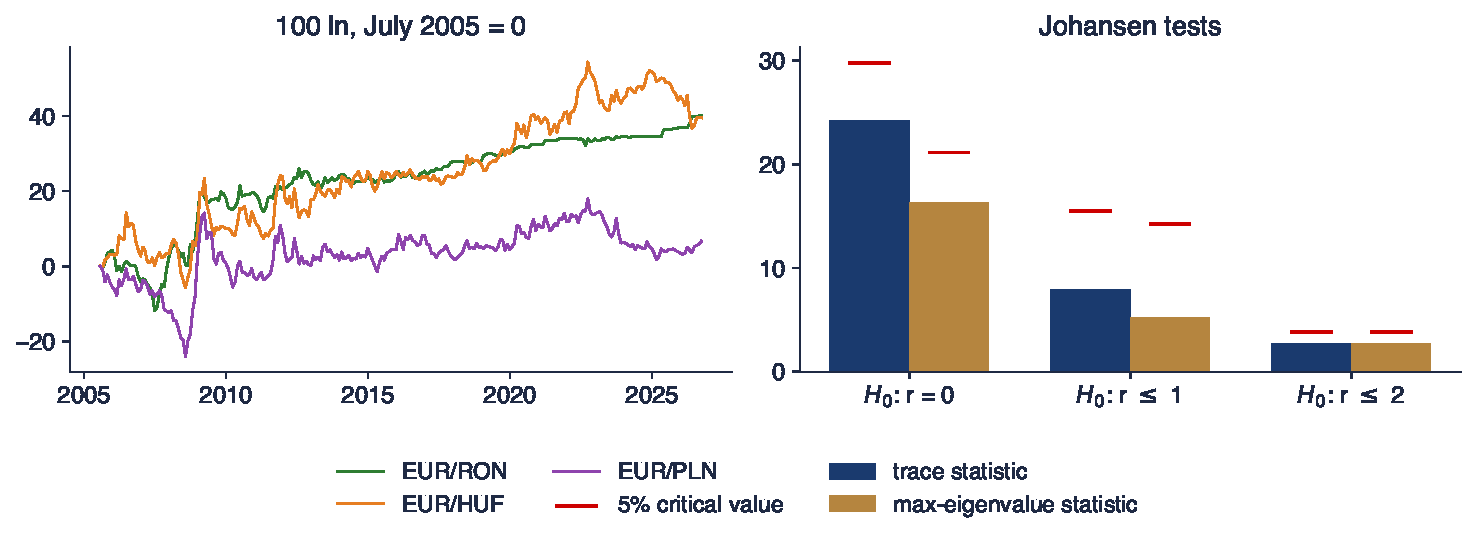
\includegraphics[width=0.96\textwidth,height=0.32\textheight,keepaspectratio]{ch7_sem_b3.pdf}
\end{center}
\vspace{-2mm}
\begin{center}
\scriptsize
\begin{tabular}{lccc}
\toprule
& $r = 0$ & $r \le 1$ & $r \le 2$ \\
\midrule
urma (valoarea de 5\%) & 24{,}21 (29{,}80) & 7{,}94 (15{,}49) & 2{,}72 (3{,}84) \\
valoarea proprie maximă (valoarea de 5\%) & 16{,}27 (21{,}13) & 5{,}21 (14{,}26) & 2{,}72 (3{,}84) \\
\bottomrule
\end{tabular}
\end{center}
\begin{itemize}
    \item ADF p = 0{,}55; 0{,}75; 0{,}08: trei cursuri $I(1)$; Johansen ($T = 255$, $k = 1$): nicio statistică nu depășește valoarea critică: rangul 0
    \item Engle--Granger p = 0{,}29 (RON, HUF), 0{,}08 (RON, PLN), 0{,}20 (HUF, PLN); corelația este 0{,}89 în niveluri, dar doar 0{,}31 în variațiile lunare
    \item Interpretare: nu; cu rangul 0 nu există niciun $\beta$ de estimat; modelăm variațiile cu un VAR în diferențe (\tsachlink{https://danpele.github.io/Time-Series-Analysis/RO/Cursuri/capitol6_modele_var_cauzalitate_granger.pdf}{Capitolul 6})
\end{itemize}\quantlet{TSA\_ch7\_seminar}{\qlurl{TSA_ch7_seminar}}
\end{frame}

\begin{frame}{B4: ROBOR, randamentul la 10 ani al României și Euribor [Propus]}
\itemsize{\footnotesize}
\begin{itemize}
\item \textbf{Întrebarea}: cîte relații pe termen lung leagă ratele dobînzii din România între ele și de Euribor și care rată se ajustează?
\item \textbf{Date}: ROBOR 3M și Euribor 3M (Eurostat), randamentul la 10 ani al României (media lunară a datelor zilnice), ianuarie 2010--august 2026; model: B3
\item \textbf{Cerințe}
\begin{enumerate}
    \item Aplicați testele Johansen (constantă, decalaje după BIC) și alegeți rangul.
    \item Estimați VECM cu acest rang și cu constanta restricționată la relația de cointegrare; normalizați $\beta$ pe ROBOR.
    \item Raportați $\hat\alpha$ cu statisticile $t$ și aplicați ADF pe eroarea de echilibru.
    \item Interpretare: care rate sînt slab exogene și ce spune acest lucru despre condițiile monetare din România?
\end{enumerate}
\item \textbf{Raportați}: un tabel cu statisticile Johansen, $\hat\beta$, $\hat\alpha$ cu $t$, un test ADF și două fraze
\item Notebook: secțiunea B4
\end{itemize}
\end{frame}

\ifsolutions
\begin{frame}{B4: rezolvare [Propus]}
\itemsize{\scriptsize}
\begin{center}
\includegraphics[width=0.96\textwidth,height=0.32\textheight,keepaspectratio]{ch7_sem_b4.pdf}
\end{center}
\vspace{-2mm}
\begin{itemize}
    \item $T = 199$, $k = 1$: urma 44{,}15 $> 29{,}80$; 14{,}95 $< 15{,}49$: rangul 1 (testul valorii proprii maxime este de acord)
    \item $\hat\beta^\top\mathbf y_t = \mathrm{ROBOR}_t - 1{,}38\,i^{(10)}_t + 0{,}046\,\mathrm{Euribor}_t + 3{,}67$: ROBOR legat de rata pe termen lung din România; Euribor aproape absent; ADF pe eroare: p $<$\,0{,}001
    \item $\hat\alpha$: ROBOR $-0{,}159$ ($t = -4{,}72$); randamentul la 10 ani $0{,}024$ ($t = 0{,}78$); Euribor $-0{,}005$ ($t = -0{,}90$)
    \item Interpretare: randamentul la 10 ani și Euribor sînt slab exogene; ROBOR face ajustarea; rata pe termen lung reflectă inflația și primele de risc; Euribor nu este ancora ratelor de pe piața monetară din România
\end{itemize}\quantlet{TSA\_ch7\_seminar}{\qlurl{TSA_ch7_seminar}}
\end{frame}
\fi


%=============================================================================
\section{Partea C: întrebări deschise și critica unui răspuns AI}
%=============================================================================

\begin{frame}{C1: pairs trading pe două bănci [Propus]}
\itemsize{\footnotesize}
\begin{itemize}
\item \textbf{Întrebarea}: ar fi cîștigat bani un investitor care ar fi găsit Banca Transilvania și BRD cointegrate la sfîrșitul lui 2021?
\item \textbf{Date}: prețuri zilnice ajustate, formare 2014--2021, tranzacționare ianuarie 2022--septembrie 2026; modele: B1, B3
\item \textbf{Cerințe}
\begin{enumerate}
    \item Pe perioada de formare, aplicați Engle--Granger și Phillips--Ouliaris (TLV pe BRD) și păstrați $\hat b$, media și abaterea standard a spread-ului.
    \item Pe perioada de tranzacționare, aplicați regula: deschidere la $|z| > 2$, închidere la $z = 0$; calculați randamentul anual brut și net (după un cost de 0,20\% pe unitatea tranzacționată).
    \item Repetați testul Engle--Granger doar pe perioada de tranzacționare.
    \item Interpretare: este rezultatul o dovadă că pairs trading funcționează la BVB?
\end{enumerate}
\item \textbf{Raportați}: două teste, numărul de tranzacții, două randamente și un plan de proiect
\item Notebook: secțiunea C1
\end{itemize}
\end{frame}

\ifsolutions
\begin{frame}{C1: analiză de referință [Propus]}
\itemsize{\scriptsize}
\begin{center}
\includegraphics[width=0.96\textwidth,height=0.32\textheight,keepaspectratio]{ch7_sem_c1.pdf}
\end{center}
\vspace{-2mm}
\begin{itemize}
    \item Formarea: $\hat b = 1{,}49$, Engle--Granger p = 0{,}028, Phillips--Ouliaris p = 0{,}065: cointegrate la 5\% doar după un test
    \item Tranzacționarea: 3 tranzacții; brut 5{,}93\% pe an (Sharpe 0{,}68), net 5{,}67\% (Sharpe 0{,}66); spread-ul a coborît pînă la $z = -4{,}40$ înainte să revină
    \item Doar pe 2022--2026: Engle--Granger p = 0{,}12, panta 1{,}19: relația s-a slăbit; în eșantion, cu parametrii întregii perioade: 3{,}30\% pe an
    \item Interpretare: nu; 3 tranzacții sînt o anecdotă, perechea a fost aleasă a posteriori, iar un spread la $z = -4{,}40$ ar fi putut continua să scadă; Cursul 7 testează 28 de perechi cu ferestre mobile
    \item Proiect: pairs trading la BVB cu selecție pe ferestre mobile, mai multe praguri, costuri realiste și limite ale vînzării în lipsă
\end{itemize}\quantlet{TSA\_ch7\_seminar}{\qlurl{TSA_ch7_seminar}}
\end{frame}
\fi

\begin{frame}{C2: verificați un răspuns AI [Propus]}
\itemsize{\scriptsize}
\begin{itemize}
    \item Un student a întrebat un asistent AI despre cointegrare. Răspunsul:
    \item \aiprompt{(a) Statistica Engle-Granger este -3,0 cu două variabile; deoarece -3,0 < -2{,}87, valoarea Dickey-Fuller de 5\%, seriile sînt cointegrate.}
    \item \aiprompt{(b) Coeficientul erorii de echilibru decalate din ECM este +0,15, deci 15\% din distanță se corectează în fiecare perioadă.}
    \item \aiprompt{(c) Johansen respinge r = 0 și r <= 1, dar nu și r <= 2 pentru trei randamente, deci randamentele au două trenduri comune.}
    \item \aiprompt{(d) EUR/RON și EUR/HUF sînt ambele I(1), iar R2 = 0{,}79 în niveluri, deci sînt cointegrate.}
    \item \aiprompt{(e) Dacă două serii sînt cointegrate, cel puțin una dintre ele o cauzează Granger pe cealaltă.}
    \item \aiprompt{(f) O regulă de pairs trading cu raportul Sharpe 0,44 pe datele din 2014-2026 își va păstra acest raport Sharpe și în viitor.}
    \item Cerințe
    \begin{itemize}
        \item 1. Pentru fiecare afirmație, precizați dacă este corectă; dacă nu este, formulați afirmația corectă și, acolo unde se poate, dați valoarea corectă din notebook (secțiunea C2).
        \item 2. Raportați: o listă de șase verdicte, fiecare cu un rînd de justificare.
    \end{itemize}
\end{itemize}
\end{frame}

\ifsolutions
\begin{frame}{C2: rezolvare [Propus]}
\itemsize{\scriptsize}
\begin{itemize}
    \item (a) Greșit: testele pe reziduuri cer valoarea Engle--Granger, circa $-3{,}36$; $-3{,}0 > -3{,}36$: fără cointegrare la 5\%
    \item (b) Greșit: un coeficient pozitiv îndepărtează $y$ și mai mult de echilibru; corecția erorii cere un coeficient negativ
    \item (c) Greșit: rangul 2 înseamnă doi vectori de cointegrare și $3 - 2 = 1$ trend comun
    \item (d) Greșit: un $R^2$ mare între serii $I(1)$ nu dovedește nimic; Engle--Granger p = 0{,}29
    \item (e) Corect: conform teoremei de reprezentare a lui Granger, cel puțin un coeficient de ajustare este nenul, deci nivelurile decalate ajută la prognoza cel puțin a unei variabile
    \item (f) Greșit: valoarea 0,44 folosește parametrii întregului eșantion și o pereche aleasă a posteriori; în afara eșantionului, regula pe ferestre mobile cîștigă aproape zero după costuri (Cursul 7)
\end{itemize}\quantlet{TSA\_ch7\_seminar}{\qlurl{TSA_ch7_seminar}}
\end{frame}
\fi


%=============================================================================
\section{Încheiere}
%=============================================================================

\begin{frame}{Idei de reținut}
\itemsize{\small}
\begin{itemize}
    \item Testați întîi că fiecare serie este $I(1)$; apoi testați eroarea de echilibru, niciodată corelația nivelurilor
    \item Testele pe reziduuri cer valorile critice Engle--Granger, care depind de numărul de variabile
    \item ECM dă viteza de ajustare; timpul de înjumătățire $\ln 0{,}5/\ln(1 + \gamma)$ este în unitățile datelor
    \item Johansen dă rangul; $n - r$ este numărul trendurilor comune; $\alpha$ arată cine se ajustează
    \item Un răspuns AI este o ciornă: verificați valorile critice, semnele și numărul trendurilor
\end{itemize}
\end{frame}

\begin{frame}{După seminar}
\itemsize{\small}
\begin{itemize}
    \item Cursul 7 dezvoltă fiecare temă de azi: trendurile comune, distribuția Engle--Granger, ECM, modelul VECM și teorema de reprezentare a lui Granger, testele Johansen, prognoza și pairs trading
    \item Încercați cerințele [Propus] în notebook
    \item C1 poate deveni un proiect de echipă: pairs trading la BVB, în afara eșantionului și după costuri
    \item Lectură: \refHP, cap.~9; \refHamilton, cap.~19--20; \refEG
    \item \textbf{Seminarul are rol de exercițiu și nu se notează; rezolvările cerințelor [Propus] se discută la seminar}
\end{itemize}
\end{frame}


%=============================================================================
\section{Bibliografie}
%=============================================================================

\begin{frame}{Bibliografie}
\itemsize{\tiny}
\begin{itemize}
    \item Engle, R. F., \& Granger, C. W. J. (1987). Co-integration and error correction: Representation, estimation, and testing. \textit{Econometrica}, 55(2), 251--276. \href{https://doi.org/10.2307/1913236}{doi:10.2307/1913236}
    \item Gatev, E., Goetzmann, W. N., \& Rouwenhorst, K. G. (2006). Pairs trading: Performance of a relative-value arbitrage rule. \textit{Review of Financial Studies}, 19(3), 797--827. \href{https://doi.org/10.1093/rfs/hhj020}{doi:10.1093/rfs/hhj020}
    \item Hamilton, J. D. (1994). \textit{Time Series Analysis}. Princeton University Press. \href{https://doi.org/10.2307/j.ctv14jx6sm}{doi:10.2307/j.ctv14jx6sm}
    \item Huang, C., \& Petukhina, A. (2022). \textit{Applied Time Series Analysis and Forecasting with Python}. Springer. \href{https://doi.org/10.1007/978-3-031-13584-2}{doi:10.1007/978-3-031-13584-2}
    \item Johansen, S. (1988). Statistical analysis of cointegration vectors. \textit{Journal of Economic Dynamics and Control}, 12(2--3), 231--254. \href{https://doi.org/10.1016/0165-1889(88)90041-3}{doi:10.1016/0165-1889(88)90041-3}
    \item Johansen, S. (1991). Estimation and hypothesis testing of cointegration vectors in Gaussian vector autoregressive models. \textit{Econometrica}, 59(6), 1551--1580. \href{https://doi.org/10.2307/2938278}{doi:10.2307/2938278}
    \item MacKinnon, J. G. (2010). Critical values for cointegration tests. Queen's Economics Department Working Paper No.~1227, Queen's University. \href{https://ideas.repec.org/p/qed/wpaper/1227.html}{ideas.repec.org/p/qed/wpaper/1227}
    \item Phillips, P. C. B., \& Ouliaris, S. (1990). Asymptotic properties of residual based tests for cointegration. \textit{Econometrica}, 58(1), 165--193. \href{https://doi.org/10.2307/2938339}{doi:10.2307/2938339}
\end{itemize}
\end{frame}

\end{document}
